\documentclass[14pt]{extbook}
\linespread{1.25}

\usepackage[utf8]{inputenc}
\raggedbottom

\usepackage[russian]{babel}
\usepackage{indentfirst}
\usepackage{misccorr}

\pdfminorversion=7

\usepackage{fancyhdr}
\pagestyle{fancy}

\usepackage{epigraph}
\renewcommand\textflush{flushright}
\usepackage{etoolbox}
\setlength\epigraphrule{0pt}
\setlength\epigraphwidth{.8\textwidth}

\usepackage[font=small,labelfont=bf]{caption}

\usepackage[pdftex]{graphicx}
\usepackage[outdir=../../out/]{epstopdf}

\DeclareGraphicsExtensions{.jpg,.png,.gif}

\usepackage[top = 4cm, bottom = 4cm, left = 3cm, right = 3cm]{geometry}
\usepackage{amsfonts}

\usepackage{multirow}

\usepackage{mhchem}


\begin{document}

\title{Математика Манхэттенского проекта}
\author{Сергей Полянских}
\date{}

\maketitle{}

\tableofcontents{}

\chapter*{Предисловие автора}

6 и 9 августа 1945 года на Хиросиму и Нагасаки были сброшены атомные бомбы общей мощностью около 35 килотонн в тротиловом эквиваленте.
Взрывы произошли в 500 метрах над землей, сформировав сильнейшую ударную волну и выделив огромное количество тепла и радиации.
Более 180000 человек погибло в момент взрыва и в последующие дни от ранений и лучевой болезни.  

Фактически, в этом уже не было необходимости. 
Вторая Мировая война подходила к своему завершению. 
Германия капитулировала, Япония была как никогда близка к капитуляции.
Атомные бомбардировки в основном были призваны продемонстрировать всему миру беспрецедентную военную мощь США. 
Мощь, явившуюся результатом, пожалуй, самого амбициозного проекта в истории науки, объединившего сотни лучших ученых своего времени - проекта ``Манхэттен''. 

Манхэттенский проект подвел черту под почти полувековыми размышлениями ученых о строении атома. 
Он получил статус национального и по сей день является по сути единственным примером столь успешного объединения лучших умов своего времени для достижения вполне практической и понятной каждому цели.

Применение атомного оружия не оставило равнодушным никого.
Весь мир от простых людей до ученых и политиков активно обсуждал нравственные и политические вопросы использования атомной энергии.
Кто-то искренне поражался силе научной мысли, освободившей энергию атома.
Другие решительно критиковали столь безответственное, по их мнению, применение полученных знаний о природе.
Руководители стран Европы, Советского Союза и Востока понимали, что США впервые в истории удалось получить в свои руки оружие беспрецедентной разрушительной силы. 
Это был именно тот эффект, на который надеялись основные заказчики атомного проекта в США - политики и военные.  
Началась ядерная гонка, продлившаяся почти полвека и не полностью оконченная и по сей день.

Отношение самих ученых к успеху атомного проекта было неоднозначным.
Многие из тех, кто призывал к созданию атомного оружия для победы над фашистской Германией и в конце концов осознал, что Германия не обладает ничем подобным, стали активно пропагандировать не использовать его и даже прекратить исследования в этой области. 
Сам Альберт Эйнштейн, подписавший в 1939 году знаменитое "письмо Эйнштейна Рузвельту" с призывом к созданию атомного оружия, позднее отчаянно критиковал его разработку и применение в военных целях.

Другие же ученые, напротив, продолжили активно работать в направлении увеличении эффективности и мощи ядерного оружия.
Кто-то не видел своей личной вины за произошедшее, другие подозревали Советский Союз в активизации работ к этом направлении.
Иные понимали, что работать бок о бок с лучшими умами своего времени и над столь масштабными проектами им, возможно, уже не придется. 
Так или иначе, после событий августа 1945 года исследовательская лаборатория в Лос-Аламосе, в которой родился проект ``Манхэттен'', после небольшой передышки начала работу над еще более смертоносным оружием - водородной бомбой.
Далеко не все подразделения трудились в прежнем составе, но и того, что осталось, вполне хватило для успешного завершения и этого проекта.  

Интересен и другой эффект событий августа 1945 года, изменивших отношение к науке и ученым в глазах простых людей.
Именно благодаря беспрецедентной эффективности и разрушительной мощи ядерного оружия репутация ученых среди простых людей взлетела до небес. 
До Манхэттенского проекта на ученых смотрели как на людей чудаковатых, но безобидных и погрязших в своих никому больше непонятных задачах. 
Образ эксцентричного ученого имел свой шарм, то и дело всплывая то в фантастической литературе, то в кино.
После Второй Мировой войны отношение к ученым изменилось кардинально.
Весь мир узнал, насколько разрушительными могут быть идеи, рождающиеся на кончике пера и университетских досках.
Человечество, на протяжении всей своей истории принимая дары науки в лучшем случае с неосознанной благодарностью, в большинстве своем просто не было готово к столь кардинальным и опасным изменениям в их жизни.
У многих возник естесственный страх перед той разрушительной мощью, которую наука без особого труда могла призвать в этот мир. 

Многое сказано и написано о Манхеттенском проекте.
Вполне понятны политические и иные причины, приведшие к началу активных исследований в области атомной физики.
Достаточно простой и понятной кажется теперь и сама физика процессов, протекающих в атомной бомбе.
Немногие страницы Манхэттенского проекта остались должным образом неосвещенными. 
Одна из таких страниц - математический аппарат и ученые-математики, сыгравшие исключительно важную роль в проекте.

В данной книге мы не рассматриваем морально-нравственные, экономико-политические и иные вопросов гуманитарного характера, неразрывно связанные с созданием и использованием атомной и водородной бомб.
Вместо этого мы сконцентрируемся на чисто научной-теоретической стороне процесса создания атомной и водородной бомб и, в особенности использованного в этой области математического аппарата.
Несомненным плюсом здесь является его крайняя выразительность и относительная простота, которую многие считают одним из главных факторов успеха Манхэттенского проекта.
Изложение материала в книге призвано . Приводимые рассуждения, выкладки, утверждения и теоремы иногда не соответствовуют стандартам строгости, принятым в современной математике. 

просто, не всегда строго .............. не всегда именно то, что было на тот момент.


[....благодарности....]

Эта книга явилась плодом многолетнего увлечения автора вопросами теории, применяемой в атомной физике. 
Искренне надеюсь, что изложение покажется простым и понятным даже читателям, не обладающим серьезной математической подготовкой, и доставит такое же удовольствие, какое испытывал я при ее написании.

------------------------ IDEAS ------------------------ 

















\chapter*{Введение}
\addcontentsline{toc}{chapter}{Введение}

Манхэттенский проект подвел выразительную черту под почти двухтысяцелетними размышлениями людей о строении атома.
Он получил статус национального и по сей день является по сути единственным примером столь успешного объединения лучших умов своего времени для достижения вполне практической и понятной каждому цели \cite{bib_mathphylhist}.

имя нарицательное, синоним концентрации научных идей и достижения прикладной цели



------------------------ IDEAS ------------------------ 

Тысячелетнее стремление человека проникнуть внутрь атома
Стремление человека познать микро- и макромир. Атомизм - Греция, Индия
Стало понятно, что пришло время совершенно новой науки.
Основные достижение физики начала XX века: история
Ущемленная роль математики, причины 
Основные достижение математики начала XX века: история. Мало кому что понятно :)
Война как катализатор науки.
Второе великое объединение: физика - использует математику
В некотором роде венец и черта - ПМ
Проект "Манхэттен": [кратко]
    история
    амбициозность
    результаты
    использование лучших мировых ученых
    результаты
    влияние на науку и технику в будущем
Советский атомный проект - тоже сила мысли и пр.
Описание источников - другие книги и пр.
Описание глав
Пара слов о задачах и ответах



вырос из страха перед Германией
многие лучшие умы - беженцы из захваченных Германией территорий, некоторые потеряли семьи [описать]
ученые сами искали встечи с политиками, убеждали, что смогут построить супероружие
даже когда стало понятно, что Германия к концу войны по сути только приступила с создании супероружила ...  запущенная машина уже не могла остановиться, предостережения ученых уже не слушали
военные опасались только  одного - скорой капитуляции Японии и всеми силами стремились успеть сбросить бомбы до окончания втрой мировой войны

состав МП в итоге оказался поистине звездным [раскрыть]

Во всем обилии имеющейся информации по МП плохо прослеживается, пожалуй, лишь один мотив - роль в нем выдающихся математиков и математики как науки.
А она была колоссальна.
Сама специфика поставленной перед учеными МП задачи была такова, что новая физика атома говорила на языке математики на совершенно новом , разработанном незадолго до этого - функциональном анализе.
Более того, основной источник информации в физике - эксперименты - были просто недоступны в большом количестве из-за крайне дорогого рабочего материала - ??? - 
и крайне высокого уровня опасности проведения любых экспериментов с ним. Подобные эксперименты стоили жизни по меньшей мере двум физикам МП - ???

именно благодаря этим факторам, модели и объяснения, даваемые математиками МП, сыграли выдающуюся роль при создании сначала атомной, а затем и водородной бомб. 
Роль, которая осталась за кадром как наиболее трудно объяснимая и лишенная той прямолинейной романтики, которой обрасла роль физика-ядерщика посла второй мировой войны.

Последствия также были .... - разделы теорвера - ветвящиеся процессы, метод Монте-Карло - основа вероятностного вывода, основы вычислительной математики и кибернетики, [еще].

благодаря усилиям таких мировых величин науки как Дж. фон Нейман были созданны первые электронные вычислительные машины, роль которых и в самой войне и впоследствии переоценить сложно.
первые компьютеры были размером ...
не будет преувеличением сказать, что весь окружающий нас сегодня цифровой мир в значительной степени взял свое начало именно тогда
  
Есть еще один довольно интересный и несколько неожиданный фактор - прикладная часть математики МП была сравнительно простой. 

детали BigBoy, FatMan , детали современного автомобиля.


Спекулируя аналогией с известным в квантовой механике принципом неопределенности Гейзенберга, можно сказать, что при описании любого явления реального мира невозможно полностью уйти ни от физики явления, ни от стоящей за ней математики.
Чем более логически строже будет изложение, тем более высокий математический уровень будет требоваться от читателя.
Напротив, желание вовсе избавиться от математики скорее всего приведет к скомканному изложению, похожему на гору взятых с потолка фактов, которые предлагается принять на веру.











XX век был поистине богатым научными открытиями в самых разных областях науки. Ученые как никогда приблизились к пониманию механики как микро, так и макро процессов окружающего мира. В биологии был обнаружен и описан основной строительный блок всего живого - молекула ДНК. Стремительно начала развиваться генная инженерия, находя приложения в самых разных отраслях человеческой деятельности. В физике были открыты общая и специальная теории относительности, квантовая механика. Выдающиеся достижения физиков и биологов активно освещались в прессе и практически сразу становились предметом жаркого обсуждения даже людьми, далекими от мира науки и в лучшем случае довольно приблизительно понимающими, о чем идет речь. 
Подобного, к сожалению, нельзя сказать об отношении к достижениям математики XX века - кроме самих математиков и, пожалуй, некоторых физиков, о них не знал практически никто. А они были поистине впечатляющими, вполне сравнимыми по потенциальной мощи с квантовой механикой или открытием ДНК. Стоит упомянуть хотя бы появление и активное использование компьютеров, необходимых для сложных расчетов тогда и распространенных повсеместно сейчас.

Отсутствие должного освещения открытий математики отчасти связано с самой спецификой данной науки. Лишь в редких случаях по-настоящему сложную математическую теорию можно объяснить широкому кругу людей-непрофессионалов. Чувство красоты математических рассуждений, доказательств и окончательных выводов необходимо упорно воспитывать в себе некоторое время, прежде чем появится понимание того, что стоит за длинными формулами и придет осознание того, как полученные выводы можно применить на практике.
Данная книга призвана восполнить этот пробел и рассказать, какую роль сыграли математики в знаменитом манхэттенском проекте, явившим миру всю мощь ядерной энергии. Я попытаюсь осветить мат. аппарат, который использовался при расчетах, связанных с конструированием атомной и водородных бомб, уделяя особое внимание методам, созданным именно в процессе работы над проектом “Манхэттен”.



Формулу $E = mc^2$ как мантру может повторить практически любой современный человек.
Многие из нас так или иначе слышали о ней еще в детстве, не подозревая, что же она в действительности означает.
....


Попытки разобраться в сути какого-либо уже исследованном кем-то ранее явлении реального мира чем-то напоминают процесс очистки гипотетического фрукта с многослойной кожурой.
Первым и самым простым слоем являются личный опыт, мнения других людей и ``авторитетных'' источников о данном вопросе. 
На этом, собственно, можно и остановиться, сказав, что достаточно разобрались в вопросе.

Если полученные ответы нас не устраивают, не понятны, либо не полны и желание разобраться в сути явления не угасло, то придется перейти к следующему слою - предметной области явления, например, физике.
Необходимо хотя бы в общих чертах понять, что же именно происходит в интересующем нас явлении природы. 
Какие объекты в нем участвуют и по каким правилам взаимодействуют друг с другом. Какие моменты существенны, а какими можно пренебречь.
Продвинувшись в понимании физической сути процесса, мы 

Наконец, последний и традиционно самый трудный слой - математика явления.
Каждое явление природы имеет свой язык описания  ...  сложно .. вместо объектов - абстракции, вместо простых правил взаимодействия - сложные уравнения.



\chapter{Сила мысли}\label{ch:power_of_thought}

\epigraph{\emph{... принципиальный вопрос, почему в материальном мире мы снова и снова встречаем повторяющиеся формы и качества}}
{Вернер Гейзенберг}


Математика, используемая в базовых моделях ядерной физики, в целом не очень сложна.
Можно было бы сразу перейти к сути вопроса, как это обычно и делается в книгах по математическим вопросам ядерной физики.
Такой подход имеет свой смысл.
Дело в том, что оформившаяся математическая теория того или иного процесса вполне может быть изложена отдельно от своего физического контекста.
И тем не менее на начальном этапе математику, стоящую за ядерной физикой, не стоит пытаться рассматривать в отрыве от самого ее предмета - атома.
Для полного понимания используемых моделей крайне полезно иметь хотя бы общие представления как об основах ядерной физики, так и о сложном пути, который прошла эта прекрасная наука.

Это на самом деле довольно серьезная причина, мотивирующая оглянуться на историю какой-либо крупной научной теории, будь то атомная физика, генетика или, скажем, теория вероятностей.
Разбираясь в ее истории, понимаешь, насколько просты и естесственны были лежащие в основе самые первые идеи и насколько увлекательным был пусть к истине. 
Изначально простая теория уже потом обростала многочисленными подробностями и уточнениями, сложными математическими моделями и изощренными экспериментами, нередко стоящими огромных денег.
Если начать с конца и заглянуть в серьезные научные монографии, то любая теория может показаться неприступной и доступной лишь узкому кругу избранных.  
Но это не так.
Лежащие в основе идеи почти всегда очень просты и лежат на поверхности.

В данной главе мы постараемся в общих чертах проследить извилистый путь идеи об атоме от туманных философских догадок древности вплоть до современной точки зрения. 
У нас нет цели погружаться в историко-философские вопросы атомизма.
Мы наметим лишь общий ход его истории как мировоззрения, останавливаясь только на наиболее ярких идеях и открытиях.


\section*{Первые идеи}

Главная задача науки - получение объективных знаний об окружающем нас мире.
С древнейших времен человек пытался проникнуть в суть явлений мира по трем фронтам: в масштабах, сравнимых с обычными бытовыми, в глобальных масштабах всей вообразимой Вселенной и в наименьших масштабах, какие только можно себе представить.

Проще всего было получать знания об устройстве объектов средних размеров - с ними зачастую несложно экспериментировать.
Накапливать факты об огромных объектах уже сложнее, но все еще было вполне реально даже в древние времена - астрономия как наука имеет более чем 5-тысячелетнюю историю. 
О невообразимо малых объектах получать объективные знания до недавнего времени было практически невозможно из-за остутствия способов наблюдения за ними.
Для их исследования поначалу существовал только один инструмент - чистая мысль, а сама наука о микромире брала свое начало из чистой философии.

История попыток проникновения в тайны микромира насчитывает более двух с половиной тысяч лет.
Первым и основным подходом к описанию окружающих нас материальных объектов было мысленное разбиение их на минимально возможные элементы.
Вообще говоря, это универсальный метод исследования любых сложных объектов - пытаться разложить их на более простые, желательно элементарные части. 
Далее следует изучить отдельно каждую часть и то, как они взаимодействуют друг с другом.
Поэтому не столь удивительно, что ученые древности пытались найти и описать некие универсальные элементы - атомы, из которых должны состоять все объекты окружающего мира.

Начало истории об атоме теряется в древних веках.
Доподлинно неизвестно, когда и кому впервые пришла в голову знаменательная идея о том, что все наблюдаемые в природе объекты при всем многообразии их форм и свойств обязаны состоять из небольшого числа одинаковых \textit{элементарных} частиц.
Скорее всего это происходило независимо в разное время и в разных культурах.
Поначалу это были 


Наиболее хорошо восстановлен и изучен античный атомизм, но и греки переняли его от более древних цивилизаций Востока, Вавилона и, вероятно, Египта.
Важно, что именно в древней Греции атомизм заиграл всеми красками, глубоко проникая и давая плоды в философии, физике и даже самой математике.

В древности практически одновременно возникли два взгляда на атомарную структуру объектов - философский и математический.
Философский атомизм пытался описать все объекты реального мира как состоящие из некоторых элементарных неделимых частиц, движущихся в абсолютной пустоте.
Математический атомизм с самого начала носил ярко выраженный прикладной характер, служа вполне конкретной цели - точному вычислению площадей и объемов тел, представляя их в виде совокупности \textit{бесконечно малых} слоев.
Позже мы увидим (см. главу ?????), что это по сути единственный возможный способ определения \textit{меры} (площади или объема) сложного объекта - приблизить его более простыми объектами, мера которых известна.
Именно так определяют меру объектов на плоскости и в пространстве в современной математике.
Оба этих подхода, философский и математический, тесно переплетались, служа постоянными генераторами новых идей, дополняя и подкрепляя друг друга.

Истоки математического атомизма стоит искать у Пифагора и его учеников в VI веке до н.э. 
О тех временах осталось совсем немного достоверных свидетельств.
Вымыслы и легенды практически не отделимы от реальных событий.
Более-менее достоверно известно, что в центр своего учения пифагорейцы ставили целые числа.
Они считали, что все объекты Вселенной должны описываться ими или их отношениями - дробями.
По легенде, эта атомистическая числовая концепция была опровергнута одним из пифагорейцев - Гиппасом, впервые нашедшим несоизмеримые отрезки, то есть отрезки, отношение длин которых не равно никакому отношению двух целых чисел.
Неизвестно, что это были за отрезки - диагональ и сторона квадрата, правильного пятиугольника или что-то еще.
Также неизвестно наказание, которое Гиппас понес за свое открытие - смерть или простое изгнание.   
Так или иначе, атомистическая концепция в целых числах продержалась недолго, но вместе с наследием более древних народов натолкнула на правильные мысли более поздних математиков античности.

Возникновение философского атомизма в его классическом виде связывают с именами двух мыслителей античности - Левкиппа и Демокрита.
Про первого известно совсем немного.
Труды Левкиппа не дошли до нашего времени.
Некоторые историки ставят под сомнение даже само его существование, настолько мало информации о нем осталось.
Демокрит же, несмотря на множество легенд и анекдотичных историй о себе, является вполне реальной исторической фигурой. 
За свой оптимизм и привычку смеяться он был известнен как ``смеющийся философ''.
По одной из легенд, соседи, обеспокоенные постоянными приступами его смеха, вызывали к нему самого Гиппократа, который не выявил у Демокрита опасных отклонений.
По другой легенде, Демокрит ослепил себя, чтобы зрение не мешало мысли. 
Это, впрочем, считается маловероятным.
Скорее всего, зрение Демокрит потерял естественным образом, а прожил он, по разным источикам, от 90 до 109 лет.

Будучи сыном одного из богатейших жителей Абдер - города на севере Греции, Демокрит получил прекрасное образование.
Большую часть юности и наследства он потратил на путешествия, впитывая знания Древнего Египта, Индии, Персии и Вавилона.
По собственному выражению, он ``объездил больше земли, чем кто-либо из современных ... людей, подробнейшим образом исследуя ее''.
Интересно, что за подобные растраты его по закону Абдер ждало наказание.
Однако по легенде, Демокриту удалось склонить судей на свою сторону, зачитав им отрывок одной из книг, написанных во время путешествий.
Судьи сочли подобный труд достойным оправданием и не стали наказывать Демокрита за растрату наследства. 

Демокрит по праву считается одним из основных создателей древнегреческого атомизма в его классическом виде.
Он впервые обобщил имеющиеся древние знания и выдвинул гипотезу о атоме, которая и стала впоследствии фундаментом для всей последующей науки.
Среди всех источников древности, наибольшее влияние на будущие научные интересы Демокрита, по всей видимости, оказали знания Вавилона.
Именно пленные халдеи (представители семитских племен Вавилона) передали ему среди прочего свои соображения об устройстве мира, которые он затем блестяще развил.

В основу учения Демокрита легли следующие утверждения:
\begin{itemize}
    \item Вселенная состоит из \textit{Великой Пустоты} и бесконечного множества \textit{атомов} - неделимых частиц, различных по форме и размеру, но неразрушимых, абсолютно однородных и непроницаемых.
    \item Атомы взаимодействуют друг с другом путем случайных столкновений, являющихся причиной всех остальных движений. 
    \item Все объекты мира состоят из конечного числа атомов.
    \item Никакие объекты не возникают из ничего и не исчезают бесследно, только путем комбинации или распада других объектов.
\end{itemize} 
Эти мысли, пока еще чисто философские, стали важной вехой не только философии, но и всей науки в целом.
Несмотря на игнорирование и даже явную критику философии Демокрита признанным тогда научным авторитетом Платоном, атомизм выдержал испытание временем и в итоге лег в основу всей современной физики и химии.

В свою очередь, идеи математического атомизма, рассорившие адептов крупнейшей античной математической школы Пифагора, послужили хорошей почвой для новых идей как философии, так и в самой математике.
Через некоторое время они были существенно развиты и с успехом использовались Евдоксом, а затем и самим Архимедом.

Арихимед, великий ученый античности, получил прекрасное образование в Александрии - одном из крупнейших научных центров того времени. 
Там он среди прочего изучал труды Демокрита и Евдокса, откуда и узнал об идее атомизма в ее математической и философской интерпретациях.
Фактически только из трудов Архимеда и можно узнать об античном атомизме, так как все, что было до него, по большей части утеряно.
Сам Архимед использовал концепцию математического атомизма в виде значительно усовершенствованной им более ранней \textit{идеи равносоставленности} Евдокса.

\begin{figure}[t!]
   \centering
   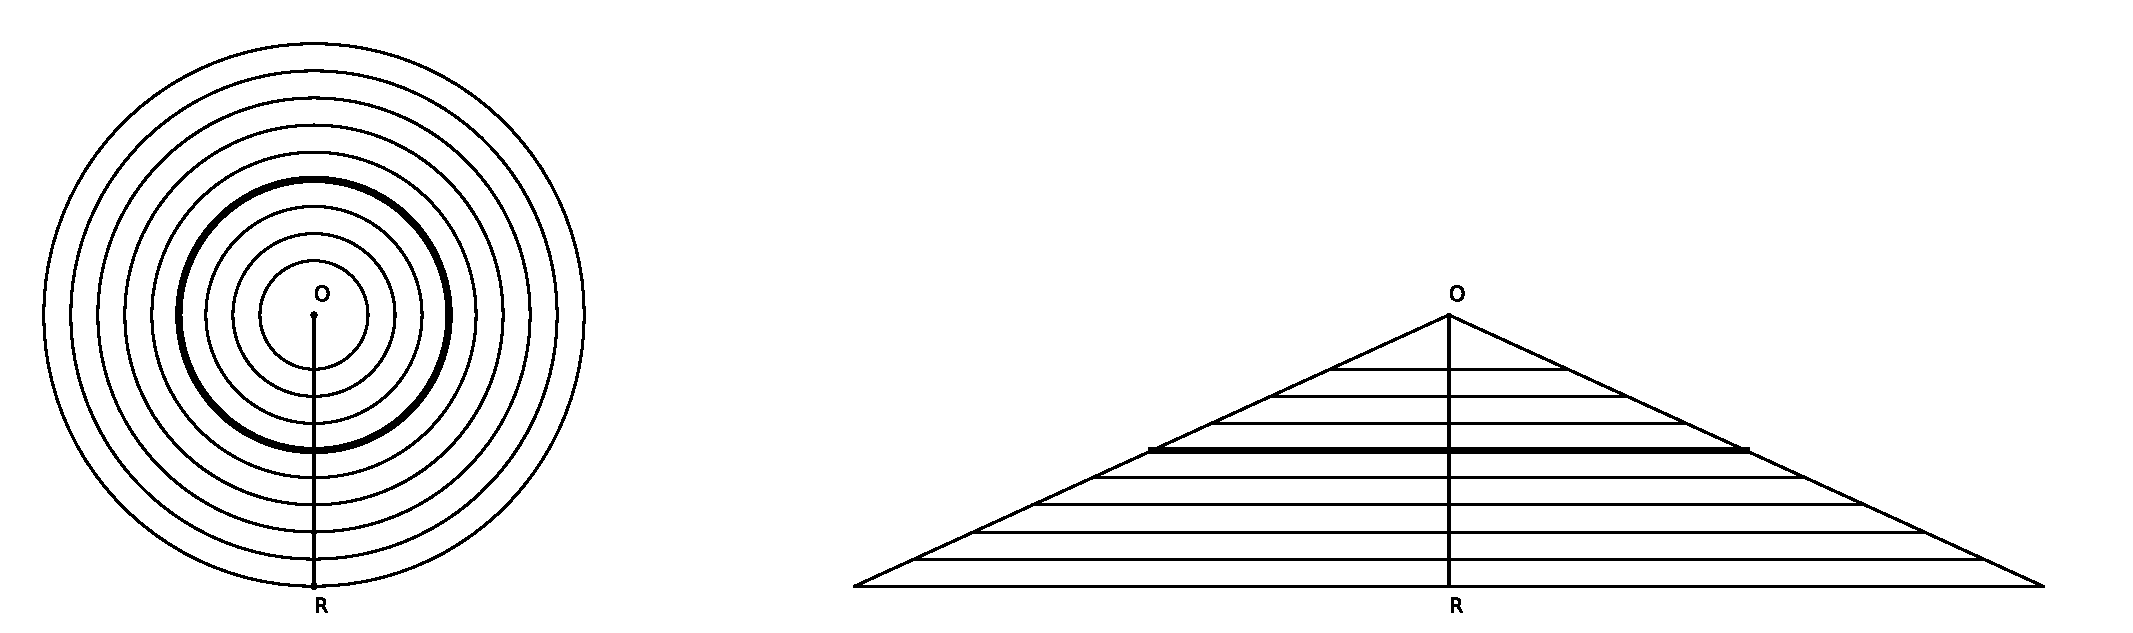
\includegraphics[scale=0.44]{images/archimed_1}
   \caption{Равносоставленность круга и треугольника.}
   \label{fig:archimed_1}
\end{figure}

Идею равносоставленности можно проиллюстрировать на следующем примере (см. рис. \ref{fig:archimed_1}).
Рассмотрим круг радиуса $R$ на плоскости.
Постараемся найти его площадь, зная что длина окружности есть произведение $2\pi$ на ее радиус.
Представим круг состоящим из неделимых объектов - концентрических окружностей с центром в центре круга.
Далее мысленно разрежем круг вдоль вертикального радиуса $OA$ и развернем каждую окружность в отрезок, сохранив ее длину и положение середины на нижнем радиусе $OR$.
В результате получится треугольник с основанием $2\pi R$ и высотой $R$.
По известной формуле, его площадь равна
\begin{equation}\label{eq:ball_square}
S = 2\pi R\cdot\frac{R}{2} = \pi R^2.
\end{equation}
Заметим, что исходный круг и полученный треугольник \textit{равносоставленны}: каждой внутренней окружности круга однозначно соответствует горизонтальный отрезок треугольника, причем той же самой длины.
Так что можно ожидать, что найденное значение \ref{eq:ball_square} равно искомой площади круга, что действительно верно.

К сожалению, принцип равносоставленности в такой интерпретации годится только для отдельных случаев и в целом неверен. 
Несложно придумать, как говорят в математике, \textit{контрпример} рассуждений подобного рода, приводящим к совершенно неверным результатам.
Интересно, что и сам Архимед не относился к этому методу как к строгому, вероятно зная, что он может привести к ошибкам.
Архимед использовал его скорее как способ угадать правильный ответ, который затем тщательно проверял.
И тем не менее, отношение к идее атомизма как конкретному математическому инструменту (пусть и не идеальному) позволило античным ученым заложить основы современного интегрального исчисления, а вместе с ним и значительной части современной математики.

В древние времена и далее в Средневековье и Новое время математический атомизм зарекомендовал себя как крайне эффективный и точный инструмент для самых разных вычислений в любых науках, где только возникали числа. 
Он стал основой для всей последующей математики как науки.
Практически весь аппарат математического анализа, развитого позднее в трудах Ньютона, Лейбница, Кеплера, Лапласа и многих других выдающихся ученых, так или иначе можно считать развитием идей Архимеда и Евдокса.
Даже беглый обзор этих достижений занял бы не одну главу и далеко увел бы нас от основного предмета книги - атома как физического объекта.
Здесь мы должны отвлечься от математического атомизма и вернуться к атомизму философскому, так как именно он дал начало физике атома.


Идеи раннего атомизма, конечно же, были довольно далеки от современного взгляда на вещи.
И тем не менее кажется удивительным то, как далеко удалось продвинуться в своих размышлениях философам древности, не обладавшим серьезными измерительными приборами и даже целенаправленно избегавшим экспериментов, доверяя лишь чистой мысли.
Даже те начальные знания, полученные учеными древности практически только силой мысли, имеют прямые параллели с самыми современными взглядами на вещи.
При должной фантазии в философских учениях восточной и греческой философии вполне можно увидеть намеки на современное представление о микромире.
В буддизме, например, с древних времен фактически фигурировал вакуум как материальная среда, в которой мельчайшие частицы непрерывно возникают и исчезают. 
Сегодня подобный взгляд на вещи составляет основу квантовой теории поля, согласно которой так называемые \textit{виртуальные частицы} ведут себя схожим образом. 
Атомы по Демокриту участвовали в непрерывных случайных столкновениях друг с другом, порождая всевозможные движения объектов. 
Последнее весьма похоже на описание броуновского движения, если считать атомы Демокрита современными молекулами.

Античный период в истории характеризуется общим расцветом культуры, искусства, философии и естественных наук.
Активно развивались астрономия, математика, из философии понемногу выделялась физика как самостоятельная экспериментальная наука.
К сожалению, за резким подъемом последовал резкий и продолжительный упадок, грозивший полной или частичной утратой древних знаний.
Не обошла эта участь и философию атомизма.
В период раннего Средневековья он фактически находился под запретом господствующей религии и чуть не был утерян совсем.


\section*{Средневековье}

Атомизм был довольно популярен в античности, но в средние века уступил взглядам Платона и Аристотеля, частично поддерживаемым набирающим силу христианством.
Лишь в X веке к философии Демокрита стали постепенно и осторожно возвращаться.
Примечательно, что происходило это именно в христианских монастырях Англии, Ирландии и Франции.
В то время спорить с доминирущими религиозно-политическими устоями можно было лишь пассивно и обладая достаточным уровнем влияния, то есть по факту быть не только ученым, но в первую очередь и священнослужителем высокого ранга.
Как и в античности, такие авторитеты определялись весьма редким сочетанием хорошей финансовой обеспеченности и тяги к знаниям.

Одними из первых влиятельных покровителей науки в Средневековье стали Герберт Аврилакский и его ученик Фульберт Шартрский.
Герберт был ученым и видным церковным и политическим деятелем.
Он с детства интересовался наукой и получил отличное по тем временам образование, проводя время за изучением достижений арабской и древнегреческой математики, астрономии и философии.
Вместе с этим он сделал блестящую карьеру в церкви, быстро став архиепископом, а затем и папой Сильвестром II.
Используя свое значительное влияние и сохранив приобретенную в юношестве тягу к знаниям, Герберт сыграл выдающуюся роль популяризатора науки в целом и философии атомизма в частности.
Именно благодаря нему монастыри снова стали основными центрами просвещения своего времени.

При жизни Герберта, даже будучи Папой Сильвестром II, неоднократно обвиняли в колдовстве, отступничестве от христианской веры и других грехах, выдумывая красочные легенды на этот счет.
По одной из таких легенд, Герберт с помощью черной магии создал медную голову, умевшую односложно отвечать на все его вопросы и помогавшую ему избегать опасности.
В другом варианте этой легенды, магическую голову вручили ему последователи тайного индийского культа.
Даже за малую часть того, что рассказывали о Герберте обычный человек в то время вполне мог поплатиться жизнью.
Можно только вообразить себе, каким влиянием нужно было обладать, чтобы не только успешно избегать прямого конфликта с недругами, но и продолжать играть роль просветителя в те темные времена.

Многое для развития науки и образования в XI веке сделал французский ученый и теолог Фульберт Шартрский, которого при жизни сравнивали с Сократом.
Будучи епископом, он превратил Шартрский собор в центр преподавания философии, наук и искусств.
Особое внимание уделялось математике.
Философам Шартрской Школы атомизм обязан своим возрождением не в меньшей степени, чем Герберту Аврилакскому.

Благодаря усилиям Герберта, Фульберта и других ученых священнослужителей Средневековья частично утраченные и забытые знания снова становились доступными для изучения и обсуждений.
Науки Востока и античности постепенно возрождались после почти 1000-летнего забвения.
Возвращалась сама культура логических рассуждений, а вместе с ней и истинно научный способ получения новых знаний.

Открыто об идеях Демокрита заговорили лишь еще через 700 лет.
Последней яркой фигурой средневекового атомизма стал католический священник Пьер Гассенди, фактически воскресивший его на рубеже Средневековья и Нового времени.
Гассенди был во многом выдающейся личностью своего времени. 
Аббат и профессор теологии в юношестве и профессор математики впоследствии, помимо богословия активно интересовался физикой, астрономией и математикой. 
Десятиления упорного труда ушли у него на восстановление забытых или запрещенных ранее трудов древнегреческих философов. 
Принятая Гассенди точка зрения на атомизм во многом повторяла учение Демокрита о пустом пространстве и существующих в нем неделимых элементах материи - атомах. 
Он добавил к классическому атомизму один очень существенный элемент - в 1647 году впервые ввел в науку понятие \textit{молекулы} как соединения отдельных атомов. 
Гассенди пришел к верному выводу, что все тела состоят из молекул, и именно молекулы определяют их основные свойства.

Идея о молекулярном строении тел не была далеко развита самим Гассенди, но высоко ценилась выдающимися учеными Нового времени - Бойлем и Ньютоном.
Именно Бойль под влиянием молекулярной теории Гассенди впоследствии развил свою теорию, объясняющую физические и химические явления в газах.    

Распространение учения об атоме в Средневековье во многом обязано отдельным выдающимся личностям, пытавшимся примирить его с религией.
Спорить с господствующей более тысячи лет догмой могли только влиятельные религиозные и политические фигуры, но даже они довольно сильно рисковали.
Хотя нет прямых свидетельств жестокого преследования атомизма со стороны инквизиции, учение это было крайне непопулярно.
Его приверженцам зачастую приходилось приносить долгие официальные извинения.

Ценность эпохи Средневековья для атомизма заключается не столько в конкретных достижениях, сколько в самом факте того, что он не был утерян совсем и продолжил свое развитие далее, в Новое время.


\section*{Новое время}

Конец эпохи Средневековья характеризовался постепенным снятием религиозных запретов на целые области древних и новых наук. 
Это позволило кардинально переосмыслить как имеющиеся знания, так и сам метод получения новых.
Стало ясно, что внимания достойны лишь те факты и наблюдения, которые можно повторить и проверить.
Сила авторитетов древности начала уступать силе объективных знаний и основному способу их получения - научному методу.
Новая методология научного исследования, сформулированная в XVI-XVII веке Френсисом Бэконом, опиралась на следующий принцип: \textit{источником знания и критерием его истинности является только опыт, который можно повторять необходимое число раз}.

\textit{Научный метод} Бэкона устанавливал следующий процесс получения новых фактов об устройстве мира: 
\begin{itemize}
    \item наблюдение,
    \item формулировка гипотез,
    \item проведение необходимых экспериментов для их подтверждения или опровержения,
    \item проверка воспроизводимости всех полученных результатов.
\end{itemize}
Сейчас подобный подход к исследованиям кажется простым и естественным, но в то время это была настоящая революция.
До этого считалось, что ответы на все вопросы можно найти у Аристотеля.
Научный подход исключал субъективность и позволял каждому желающему убедиться в справедливости выдвинутых кем-либо теорий.
Теперь каждый мог привнести в науку что-то свое.
Нужно было лишь поставить соответствующий эксперимент, выдвинуть гипотезы и подтвердить свои догадки.

Новый подход к знаниям коснулся всех научных идей древности и в первую очередь самого атомизма.
К счастью, Средневековье не только сохранило его как систему взглядов, но и привнесло новое важное понятие молекулы, которое стало ключевым для дальнейшего понимания устройства мира. 
Теперь это понятие предстояло уточнять и строить на его основе не только качественные догадки, но и делать количественные предсказания.
Новые правила научной игры подходили для этого как нельзя лучше.
Очень скоро из собрания чисто философских идей атомизму предстояло стать прочной основой для всей современной физики и химии.

Первый шаг на этом пути был сделан ирландским ученым и богословом Робертом Бойлем.
Получив в Европе прекрасное образование, богатым наследником он вернулся в родную Ирландию, где полностью посвятил себя науке.
Бойль был не только талантливым экспериментатором, но и одним из первых физиков-теоретиков.
Вдохновившись идеями античных ученых и молекулярной гипотезой Гассенди, он смог существенно продвинуться в вопросах строения вещества. Бойль получил, по сути, первое существенное доказательство существования атомов и молекул.
А именно, опираясь на гипотезу о молекулярном строении вещества, Бойль в 1662 году впервые установил строгое математическое соотношение между объемом некоторого газа $p$ и его давлением $V$:

\begin{equation}\label{eq:boil}
pV = c.
\end{equation}

При всей своей простоте эта формула была уже не просто абстрактной философской идеей.
Она позволяла делать как качественные, так и строгие количественные предсказания.
Например, из нее следовало, что при сжатии объема с газом, давление в нем возрастает.
При этом можно посчитать, во сколько именно возрастает давление.
Более того, формула Бойля находилась в прекрасном соответствии с предположением об атомно-молекулярном строении вещества.
Действительно, если в данном ограниченном элементе объема находятся хаотически движущиеся частица газа, то при уменьшении объема давление, вызванное их соударениями со стенкой, будет возрастать.

Формула (\ref{eq:boil}) служила довольно убедительным доводом в пользу существования атомов и молекул.
Другим его значительным вкладом в науку было введение понятия \textit{химического элемента} — мальчайшей составной части простых (одноэлементных) веществ, и входящей в состав сложных.
В своих взглядах на строение веществ Бойль был уже очень близок к современному взгляду на вещи. 

Несколько позднее, в 1676 году французкий ученый Эдм Мариотт подтвердил формулу (\ref{eq:boil}), уточнив, что оно справедливо только при постоянной температуре.
Более точная формула с учетом температуры может быть записана в виде

\begin{equation}\label{eq:boil-mariott}
pV = cT
\end{equation}
с некоторой новой постоянной $c$. 
Из этого соотношения уже видно, что при повышении температуры должен возрастать объем, либо давление, и опять, эти процессы полностью описываются им количественно.
И опять, можно догадаться, что именно хаотическое движение молекул в газе ведет к увеличению его объема, давления, либо температуры.
Замечено это было позднее.
Наконец, и эта формула была уточнена до \textit{уравнения состояния идеального газа} (формула Клапейрона - Менделеева):

\begin{equation}\label{eq:klap-mendeleev}
pV = nRT.
\end{equation}
Здесь уже нет неизвестных констант.
Четкий физический смысл имеет каждая входящая в нее величина.
Эта формула связывает макроскопические характеристики газа - давление, объем и температуру с микроскопической характеристикой - количеством молекул $n$ в одном моле газа, через универсальную газовую постоянную $R$.
Важно понимать, что несмотря на отсутствие неопределенностей, формула (\ref{eq:klap-mendeleev}) тоже имеет свои границы применения.

В истории открытия формулы Бойля - Мариотта - Клапейрона - Менделеева хорошо прослеживается один очень важный принцип.
Каждая из формул (\ref{eq:boil}), (\ref{eq:boil-mariott}), (\ref{eq:klap-mendeleev}) справедлива в своих предположениях и не отменяет, а уточняет предыдущую.
Таким образом, в математической записи законов природы потенциально заложено их возможное обобщение в будущем.
По этой же причине основные уравнения квантовой механики при некоторых условиях могут быть сведены к уравнениям классической физики, а механика теории относительности Эйнштейна является не опровержением, а расширением классической механики Ньютона. 
Это очень важное свойство математических моделей.
Оно говорит о том, что даже математическое описание некоторого явления, удовлетворительно строгое в данный момент, вполне может оказаться неполным в последствии.
И это отнюдь не помешает пользоваться им сейчас и уточнить его в будущем, опираясь на новые наблюдения.

Идея молекулярного строения вещества была далее существенно развита в трудах выдающегося русского ученого М.В. Ломоносова в середине XVIII века.
Ломоносову среди прочего удалось объяснить агрегатные состояния веществ и тепловые эффекты, отвергнув господствующую теорию о теплороде - специальной субстанции, порождающей тепло.
Он пришел к заключению, что молекулы должны находиться в непрерывном движении, что и определяет тепловое состояние тел.
Как он писал, ``теплота состоит в движении материи, которое движение хотя и не всегда чувствительно, однако подлинно в теплых телах есть'' что, таким образом, устраняет ``смутные домыслы о некоторой бродячей, беззаконно скитающейся теплотворной материи''.
Свою теорию ученый подтвердил математическими расчетами и рядом блестящих для того времени экспериментов.

Молекулярно-кинетическая теория Ломоносова подвергалась жесткой критике, но в итоге стала общепризнанной вехой в атомизме.
Тем не менее, Ломоносов ошибся в ряде моментов.
Он представял молекулы шарообразными, причем тепло вырабатывалось путем их вращения, а при колебательном движении, по его мнению, тела должны были разрушаться. 
Ломоносов также не допускал, что молекулы могут соударяться друг с другом, только соприкасаться.
Эти неточности, ликвидированные впоследствии другими учеными, не говорят об ошибочности нучного метода, а скорее демонстрируют его в действии.
По словам самого ученого, ``из наблюдений устанавливать теорию, через теорию исправлять наблюдения есть лучший всех способ к отысканию правды''.
Ломоносову для описания явления распространения тепла вполне хватило правильных предположений, прекрасно подтвердившихся экспериментом.
Неверные гипотезы не помешали общим верным выводам, и были исправлены в дальнейшем, когда в этом возникла необходимость.

Следующие открытия в учении об атоме соединили атомизм с молодой наукой химией и фактически определили ее современный облик.
Они связаны с именами Джона Дальтона и Антуана Лавуазье.
Оба были выдающимися учеными своего времени.

Антуан Лавуазье был сыном состоятельного парижского адвоката. 
Параллельно с изучением юриспруденции в университете, как того хотел его отец, Лавуазье самостоятельно занимался естественными науками, чувствуя в этом свое истинное призвание.
Уже в 25 лет за свои блестящие достижения он был избран сначала адъюнктом Французской Академии наук, а впоследствии и ее действительным членом и директором.
Он внес значительный вклад в не только в химию, но также физику, физиологию и даже гуманитарные науки.

В атомизме достижения Лавуазье связаны развитием введенного Бойлем понятия \textit{элементарного тела} как химически не разложимого вещества.
Идеи Лавуазье значительным образом способствовали открытию впоследствии стехиометрических законов, то есть правил, которым подчиняются массы и объемы реагирующих веществ.
Его эксперименты были беспрецедентно точны и тщательно подготовлены.
Все это способствовало окончательному внедрению идей атомно - молекулярного строения вещества в новую тогда еще науку химию.
Именно использование понятий атома и молекулы позволяло просто и ясно объяснять химические наблюдения, что несомненно говорило в пользу их истинности.

Хотя Лавуазье не имел недостатка в средствах, личное финансовое благополучие интересовало его в гораздо меньшей степени, нежели возможность сделать новое открытие. 
Большие деньги, получаемые на государственной службе, Лавуазье тратил на эксперименты.
К сожалению, именно занимаемая им должность сборщика налогов стала для него роковой.
Ни выдающиеся заслуги перед Францией, ни непререкаемый авторитет в науке, не уберегли Лавуазье от казни по обвинению в государственной измене во время Французской революции.
Просьба Лавуазье об отсрочке своей казни на несколько дней для публикации своих последних работ была отклонена.

О преданности Лавуазье науке можно судить по следующей истории о нем.
Его волновал популярный в то время вопрос, умирает ли голова сразу после отсечения, либо живет еще какое-то время.
Накануне своей казни ученый придумал опыт, позволяющий это определить.
Согласно его задумке, в случае жизни после отсечения голова могла бы подать знак, моргнув одним глазом.  
Понимая, что проверить результаты этого опыта ему уже не удастся, он попросил это сделать палача. 
Палач оценил идею Лавуазье, но тут же заверил, что в этом эксперименте нет никакой необходимости, так как в случае мгновенной смерти казненных ему бы не приходилось время от времени менять обкусанные по краям корзины для голов.

Биограф Лавуазье, выдающийся математик Лагранж писал: ``Всего мгновение потребовалось, чтобы отрубить голову, замену которой невозможно найти и за сотни лет''.

Другой знаковой фигурой химического атомизма Нового времени был Джон Дальтон, сделавший значительный вклад в молекулярную теорию строения вещества.
За свою жизнь Дальтон совершил множество открытий, включая открытие названной его именем болезни, которой страдал сам.
Наиболее замечательными были его достижения в атомно-молекулярной теории.
С его именем, наряду с Лавуазье, связывают становление  современнойхимии как науки.

Дальтон справедливо считал, что атомы участвующих в химических превращениях веществ при химических раекциях не распадаются на части и не создаются, а лишь перераспределяются. 
Таким образом, впервые возникла идея об атоме как \textit{химически неделимом} элементе мироздания, участвующем в любом превращении веществ в природе.
В серии блестящих опытов в начале XIX века Дальтон подтвердил свою теорию.
Он обнаружил, что
\begin{itemize}
    \item давление смеси газов равно сумме давлений каждого газа в отдельности - закон парциальных давлений смесей газов,
    \item растворимость газа в жидкости пропорциональна его парциальному давлению - закон растворимости газов в жидкостях,
    \item закон равномерного расширения газов при нагревании,
    \item если два химических элемента образуют между собой несколько соединений, то отношения масс атомов одного элемента к массам атомов другого элемента между собой соотносятся как целые числа - закон кратных отношений.
\end{itemize}
Эти открытия прекрасно объяснялись атомной гипотезой строения вещества.
Так атомизм античности наконец начал обретать прочный экспериментальный фундамент.

Дальтон не остановился на указанных открытиях и сделал еще один большой шаг по направлению к современным представлениям об атоме.
Он обратил внимание на исключительную роль массы атома в химических превращениях веществ.
Дальтон впервые составил таблицу относительных атомных весов.
Таблица была очень неточна и неоднократно менялась им впоследствии.
Гораздо более точные таблицы были получены впоследствии Авогадро и Берцеллиусом (см. таблицу \ref{tab:atom_mass}).

\begin{table}
\label{tab:atom_mass}
    \begin{center}
        \begin{tabular}{|p{3cm}|p{2cm}|p{2cm}|p{2.2cm}|p{2cm}|}
            \hline
            \multirow{2}{}{Химический элемент} & \multicolumn{4}{|c|}{Относительная атомная масса} \\
            & Дальтон & Авогадро & Берцелиус & Соврем. \\
            \hline
            H & 1 & - & 1 & 1.01 \\
            C & 5.4 & 12.08 & 12.25 & 12.01 \\
            N & 5 & 13.97 & 14.19 & 14.01 \\
            O & 7 & 16.1 & 16.03 & 16.00 \\
            Ag & 10 & 216 & 216.61 & 107.87 \\
            \hline
        \end{tabular}
    \end{center}
\caption{Фрагмент таблицы атомных масс (1 а.е.м.\approx $1.661\cdot 10^{-27}$ кг).}
\end{table}

Новое время стало стало настоящим расцветом для науки.
Идеология ``идея - эксперимент - теория'' быстро прижилась в самых разных областях знаний, давая поразительные результаты.
Лаконично вписались в эту концепцию и математические методы.
Стало ясно, что законы природы должны выражаться в строгих формулах, дающих не только общее описание явления, но и возможность точных предсказаний.
Теперь можно было не только рассуждать об устройстве мира, но и применять эти знания на практике.
Это было серьезным прорывом.

Последующие открытия Нового времени, связанные с понятиями атома и молекулы, были сделаны прежде всего в физической химии. 
Они связаны с именами таких выдающихся ученых как Пруст, Авогадро, Берцеллиус, Бутлеров и Менделеев.
Описание их достижений увело бы нас от основного предмета книги - атома, в сторону химии.
Вместо этого перейдем к открытиям физики начала XX века, ставшим решающими для понимания тайн атома.


\section*{Время новой физики}

---------

Броун


---------------------------- IDEAS --------------------

История показала, насколько ...
С одной стороны, мыслители древности оказались правы - все вещества действительно состояли из небольшого числа элементарных строительных блоков.
С другой строны, само поведение атомов






\chapter{Атом}\label{ch:atom}

\epigraph{\emph{Величайшим достижением человеческого гения является то, что человек может понять вещи, которые он уже не в силах вообразить.}}
{Лев Ландау}

Идея об атоме прошла извилистый и местами весьма драматический путь, прежде чем приобрела тот вид, в котором ее изучают сегодня в школах и университетах.
Довольно простая и естественная по своей сути мысль о существовании небольшого числа первоэлементов в итоге привела к совершенно удивительным открытиям.
Все новые и новые факты об атоме, сформировавшие в начале XX века фундамент ядерной физики, поначалу скорее все больше запутывали ученых, нежели вносила ясность.
Оказалось, что знания о микромире попросту нельзя получать и интерпретировать классическим методом - используя интуицию и сравнение с какими-либо привычными объектами вроде стальных шариков или планет Солнечной системы.
Атом оказался чем-то совершенно иным.
Как писал Нильс Бор, ``если ты не шокирован квантовой физикой — ты ее еще не понял''.

Открытие и научное описание процесса деления атомного ядра стало кульминацией всей истории проникновения в тайны атома. 
Именно возможность искусственного расщепления ядер тяжелых атомов позволило освободить огромную энергию, скрытую внутри атома.
Может вызывать некоторый дискомфорт, что это по-настоящему великое открытие впервые было применено именно в военных целях.
Но таков путь истории, и его не изменить.

На протяжении всей книги нам не потребуются ни глубокие факты современной ядерной физики, ни сложный математический аппарат квантовой механики.
Для наших целей будет вполне достаточно общих знаний о строении атома и ядерных реакциях.
Без них было бы крайне тяжело понять, почему те или иные задачи ставились перед физиками и математиками Манхэттенского проекта.
Многие из них были хорошо известны ученым Манхэттенского проекта и с того времени практически не изменились.  
Этих знаний оказалось вполне достаточно для реализации основной его цели - создания ядерного оружия.
Более глубокие факты об атоме были открыты позднее и приводятся здесь лишь в самых общих чертах и только для полноты картины.


\section*{Строение}

Итак, что же такое атом? К настоящему времени известно следующее.
Атом - микроскопическая частица вещества, состоящая из тяжелого ядра, окруженного легкими по сравнению с ним электронами.
Ядро состоит из нуклонов - протонов и нейтронов.
Нуклоны в свою очередь состоят из еще более мелких субатомных частиц: глюонов, кварков и антикварков.
Эти последние частицы интересны в первую очередь тем, что наряду с электронами, вполне могут оказаться действительно \textit{элементарными}, то есть далее неделимыми на более мелкие еще неизвестные науке частицы.
Пока это точно установить не удалось.

\begin{figure}[t!]
   \centering
   \includegraphics[scale=0.5]{images/atom_1}
   \caption{Строение атома гелия: два протона и нейтрона в ядре и два электрона, ``размазанные'' около ядра в облаке формы шарового слоя. Наиболее вероятное местонахождение электронов - пунктирная сфера, но точно локализовать электрон в пространстве невозможно.}
   \label{fig:atom_1}
\end{figure}

На рис. \ref{fig:atom_1} схематически изображен атом гелия.
Он имеет два протона и нейтрона в ядре и два электрона на некотором расстоянии от центра.
В реальности электроны располагаются на очень большом отдалении от ядра - в десятки-сотни тысяч раз большем, чем его диаметр.
Само ядро атома гелия, как и любого другого элемента, в целом устроено довольно просто: протоны и нейтроны упакованы в нем довольно плотно, находясь практически в непосредственной близости друг о друга.

Число протонов в ядре $Z$ называется \textit{зарядовым числом} или \textit{атомным номером}.
Оно однозначно определяет тип химического элемента и его место в периодической таблице элементов: водород - один протон, гелий - два протона и так далее.
Полное количество $A = Z + N$ протонов и нейтронов называют \textit{массовым числом} атома.
Число электронов в атоме совпадает с числом протонов $Z$, что гарантирует его электронейтральность.

Каждый химический элемент, имея фиксированное число протонов, вполне может иметь разное число нейтронов в своем ядре.
Количество нейтронов в ядре практически не влияет на химические свойства атома.
Для одного и того же элемента с разным числом $N$ говорят о его \textit{изотопах}.
Отличаться изотопы одного элемента будут только своей массой, но не свойствами.
Главное, помимо массы, различие разных изотопов одного и того же элемента - их стабильность, о чем подробно рассказано ниже.

Обычно в природе широко распространен какой-то один изотоп каждого химического элемента.
Этот изотоп обнаруживается в подавляющем числе случаев и имеет долгое время жизни.
Остальные изотопы очень редки, либо синтезируются искусственно и имеют очень малое время жизни. 

Например, атом с одним протоном и без нейтронов в ядре представляет собой тот же самый химический элемент, что и атом одним протоном и одним, двумя или тремя нейтронами.
Это все изотопы одного и того же атома водорода: протий \ce{^{1}_{1}H}, дейтерий \ce{^{2}_{1}H}, тритий \ce{^{3}_{1}H} и квадий \ce{^{4}_{1}H}.
Самый легкий из них - протий встречается в природе в $99.98\%$ случаев.

Основной для нас пример - атом урана.
Из 26 известных его изотопов только три встречаются в природе: \ce{^{234}U}, \ce{^{235}U}, \ce{^{238}U}.
Природная смесь добываемого урана содержет в среднем $99.2745\%$ урана-238, $0,72\%$ урана-235 и $0,0055\%$ урана-234
Именно два последних имеют исключительное значение для производства ядерного оружия.
Более тяжелый \ce{^{238}U} найболее распространен в природе ($99.27\%$).
Он устойчив и не может напрямую использоваться как топливо в реакторах или рабочий материал атомной бобмы.
Наиболее ценный и гораздо более редкий \ce{^{235}U} благодаря своим свойствам может сразу быть использован в атомной бомбе, так что .....  

[подробнее о числах для Урана (отдельная секция?)]
[картинка атома урана]
[валентные эоектроны - на внешней оболочке]


\section*{Электронное облако}

Главный и наиболее сложный для понимания факт об электронах в атоме состоит в том, что их точное местоположение указать невозможно.
Они как бы размазаны в пространстве около ядра, образуя \textit{электронное облако} - довольно причудливый трехмерный объект с областями большей и меньшей плотности.

На рис. \ref{fig:atom_1} схематически изображено облако двух электронов атома гелия.
Оно представляет собой сферически симметричную область в пространстве, наиболее плотную в окрестности сферы с центром в ядре атома.
На рисунке это наиболее темная область, выделенная для наглядности пунктиром.
Сами точечные электроны на рисунке - скорее схематическая абстракция, нежели реальные точечные объекты.
Их местоположение не определено точно ни в какой момент времени - они могут находиться практически где угодно, но вероятнее всего - в более темных областях около пунктирной линии.
Подобное поведение физических объектов не встречается нигде в привычных нам наблюдаемых явлениях в обычной жизни.
Оно уникально для микромира. 

Остановимся на этом удивительном факте подробнее.
Принципиально здесь то, что неопределенность положения электрона данном случае отражает не наше субъективное незнание о местонахождении электрона, а объективный факт: положение электрона в пространстве невозможно точно определить никакими инструментами и расчетами.
Первое приходящее на ум объяснение этому факту - мы пока просто не располагаем инструментами необходимой точности, и они когда-нибудь появятся в будущем.
Но это не так.
Невозможность локализовать электрон принципиальна и никак не зависит от наших технических возможностей.

Разница между субъективной и объективной неопределенностью хорошо видна на следующем примере.
Предположим, мы подбрасываем монетку и интересуемся, какой стороной она выпадет.
Если монетка честная, то примерно в половине случаев она будет выпадать орлом, и примерно в половине - решкой.
Подбрасывая монетку, мы действительно заранее не знаем результат и говорим лишь о вероятности выпадения, например, орла.
Но в этом случае мы \textit{все-таки могли бы точно предсказать} результат, если бы знали силу и скорость броска, а также точные турбулентные движения воздуха около монетки.

С электроном все обстоит иначе.
Мы полностью лишены возможности обладания некой дополнительной скрытой информацией вроде движения воздуха вокруг монетки, которая в итоге позволила бы точно определить его местонахождение.
Ученые потратили огромное количество усилий, пытаясь найти подобные \textit{скрытые переменные}, и у них ничего не вышло.
Пришлось признать (и тому есть другие подтверждения), что электрон существует сразу везде, просто где-то с большей вероятностью. 
Распределенное в пространстве состояние - это способ существования электрона в этом мире.
Так все устроено, и ничего с этим не поделаешь. 

Смирившись с невозможностью определить точное положение электрона в пространстве, можно попытаться задаться вопросом о нахождении по крайней мере этой самой вероятности обнаружить его в определенном месте.
Так как в каких-то областях шанс обнаружить электрон выше, то должна быть возможность как-то это количественно описать.
Это, конечно, будут не точные координаты электрона, но уже и не полная неопределенность.

Для описания такого рода частичных неопределенностей в математике используются \textit{плотности распределения вероятностей} - функции, принимающие б'ольшие значения там, где вероятность должна быть выше (подробнее о плотностях см. главу….).
Таким образом, в нашем случае можно сказать, что электрон (даже один единственный!) \textit{распределен} в пространстве так, что его более вероятно обнаружить там, где значение его плотности распределения выше.
С визуальной точки зрения электронное облако электрона оказывается плотнее там, где больше его функция распределения (см. рис. \ref{fig:atom_1}).


Итак, мы связали нашу новую интуицию о положении электрона в пространстве с конкретным математическим объектом - функцией распределения вероятностей. 
Откуда же можно ее получить?
Оказывается, это вполне возможно сделать точно, решив специальное уравнение - уравнение Шреддингера  (\ref{eq:schroedinger_1}), подробнее о котором рассказано ниже.

Плотность вероятности обнаружения электрона в пространстве принято еще называть его \textit{орбиталью}.
Таким образом, математически, орбиталь является одним из решений уравнения Шреддингера.

Сделаем еще несколько замечаний относительно визуализации электронного облака, которое может быть довольно сложным трехмерным объектом.
График функции его плотности находится в четырехмерном пространстве (три пространственные координаты и еще одна ось для значений плотности), и представить его себе довольно проблематично.
Но если электронное облако, например, сферически симметрично, то о полной функции распределения вероятностей вполне можно судить по ее радиальной составляющей, то есть по ее зависимости от $r$ - расстояния до центра атома.
Так, например, для рассмотренного выше атома гелия радиальная составляющая плотности вероятности изображена на рис. (\ref{fig:radial_prob})).

\begin{figure}[t!]
   \centering
   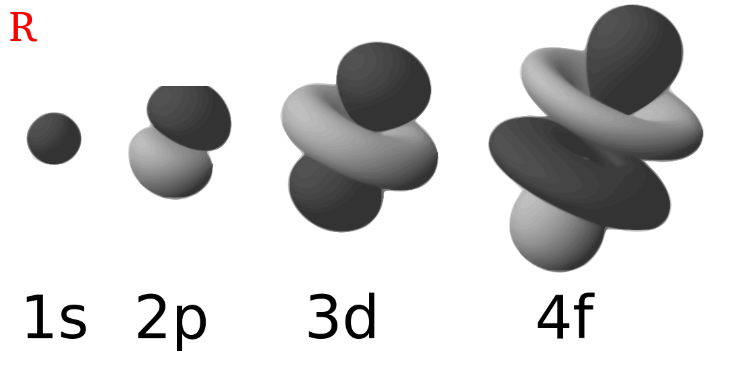
\includegraphics[scale=0.9]{images/electron_clouds_1}
   \caption{Различные виды электронных облаков.}
   \label{fig:electron_clouds_1}
\end{figure}

Иногда, желая придать положению электрона хоть какую-то конкретику, используют геометрическое представление орбитали - поверхность в пространстве, на которой плотность распределения вероятности имеет постоянное значение.
Значение выбирается либо максимальное, либо такое, что в ограничиваемой этой поверхностью области электрон может быть найден с вероятностью близкой к 1.

В случае атомов водорода и гелия эти фигуры представляют собой сферу с центром в ядре атома.
Это уже гораздо более наглядные геометрические образы, нежели абстрактные плотности распределения вероятностей.
Однако важно понимать, что они не определяют точные местоположения электрона в пространстве. 
В реальности электроны вовсе не двигаются по своим орбиталям по аналогии с движением планет Солнечной системы по своим орбитам.
Более того, само понятие движения электрона в данном случае весьма условно.
О конкретных координатах электрона, как и о траектории движения электрона по орбитали речи идти не может.

Наконец, электронное облако далеко не всегда имеет шарообразную форму.
Наиболее симметричная форма облака в виде простого шарового слоя как на рисунке \ref{fig:atom_1} может наблюдаться только у атомов водорода и гелия.
У других химических элементов формы электронных облаков гораздо сложнее и даже могут не иметь сферической симметрии.
На рис. (\ref{fig:electron_clouds_1}) изображено несколько примеров не сферически симметричных облаков.
Удивительно, но все эти замысловатые фигуры реализуются как некоторые решения уравнения Шреддингера (\ref{eq:schroedinger_1}).



\section*{Размеры}

Линейные размеры атома определить достаточно сложно из-за описанной выше неопределенности положения его электронов в пространстве.
О размерах атома принято судить либо по наиболее вероятной удаленности его электронов от ядра, либо по половине расстояния между ядрами двух одинаковых атомов в молекуле простого вещества.
В любом случае они неимоверно малы - от $31\cdot 10^{-12}$ (атом гелия) метра до $225\cdot 10^{-12}$ (атом цезия) метра.
Порядком размера атома принято считать величину $1\mbox{\normalfont\AA} = 10^{-10}$ м (ангстрем).
Понять, насколько это мало, можно учтя, что атомов в капле воды примерно $4\cdot 10^{21}$, что вполне сравнимо с числом звезд во Вселенной.

Так как нуклоны в ядре упакованы довольно плотно, то о размере ядра вполне можно судить по размеру одного нуклона - около $0.86\cdot 10^{-15}$ метра (примерно одинаковы для протонов и нейтронов). 
Таким образом, ядро в десятки - сотни тысяч раз меньше, чем весь атом.
Так, для простейшего атома водорода с диаметром порядка $53\cdot 10^{-12}$ метра и единственным протоном в ядре, электрон удален от центра на расстояние примерно в 100000 раз большее, чем само ядро \footnote{%
    Здесь, конечно же, имеется ввиду средняя удаленность электрона от ядра.
    О точном расстоянии до ядра говорить не приходится.}.
Таким образом, между протоном и электроном, где бы последний ни находился, расположено огромное количество пустоты.

Относительно размеров электрона даже в настоящее время известно очень немногое.
Последние попытки его определения показали, что оно не превосходит $10^{-20}$ метра.
В настоящее время электрон принято считать \textit{фундаментальной элементарной частицей}, то есть такой, которую пока не удалось разложить на составные частицы и определить ее размер.

В связи с этими числами обычно приводят следующий пример: если ядро увеличить до размеров теннисного мячика, то весь атом увеличится до размеров футбольного стадиона.
Электрон при этом станет не более чем песчинкой, спрятанной где-то в последних рядах стадиона без малейшего шанса его найти.

... переход

Орбитали атомов размазаны в пространстве, и невозможно точно отделить атом от окружающей его пустоты.
Более того, если учесть, что размер электронов пренебрежимо мал, а наиболее вероятные места их пребывания сконцентрированы в тонких слоях около поверхностей максимальной плотности вероятности, то электронному облаку можно не приписывать сколько-нибудь существенного объема.
Атомные ядра также имеют неимоверно малые размеры как сами по себе, так и по сравнению с размерами атомов.
Нуклоны, составляющие ядра, также не плотны, а в свою очередь состоят из более мелких \textit{фундаментальных элементарных частиц}.
Таким образом получается, что мы живем в практически пустом пространстве.


\section*{Масса}


\section*{Заряд}


\section*{Свойства}


\section*{Стабильность и распад}

Итак, атом в целом устроен довольно просто.
Но почему же он стабилен?
Чтобы атом мог существовать сколько-нибудь продолжительное время, между его протонами, нейтронами и электронами должны действовать некоторые силы.
Именно эти силы и делают атом стабильной структурой.
Эти силы не дают частицам, с одной строны, разлететься в разные строны, а с другой - упасть друг на друга.



Как было сказано выше, атомы одного и того же химического элемента всегда имеют фиксированное число протонов, но могут иметь разное число нейтронов. 
Эти обеспечивается разнообразие ...
Главное, помимо массы, различие разных изотопов одного и того же элемента - их стабильность, о чем рассказано ниже.



В среднем число нейтронов для изотопов данного химического элемента не слишком отличается от числа протонов, которое для него определено однозначно.
Число нейтронов у изотопа может быть как меньше, так и больше числа протонов.
В обоих случаях, чем больше эта разница, тем неустойчивее атом становится и тем выше вероятность ему распасться на атомы более легких элементов.
Если число нейтронов отличается от 

Выше было рассказано о неустойчивости разных изотопов и естесственной радиоактивности...
Это явления имеет ключевое значени для искусстевенного расщепления ядра атома...


Стабильность атома определяется через \textit{период полураспада} - время, за которое распадутся ядра 




Простейшим из атомов является атом водорода, обладающий минимальным числом протонов - одним.
Число нейтронов в атоме водорода может быть от нуля до семи, но с ростом их числа ядро становится нестабильным и быстро спонтанно распадается.
Так, у трития - изотопа водорода с тремя протонами, период полураспада составляет около 12 лет, а у квадия с четырьмя протонами - всего $1.4\cdot 10^{−22}$ секунды.
Это же верно для любых атомов.
Нейтроны необходимы, чтобы стабилизировать пытающиеся разлететься протоны, но с ростом их числа атом все-таки теряет стабильность (см. рис. \ref{fig:atom_stability}).


\begin{figure}[t!]
   \centering
   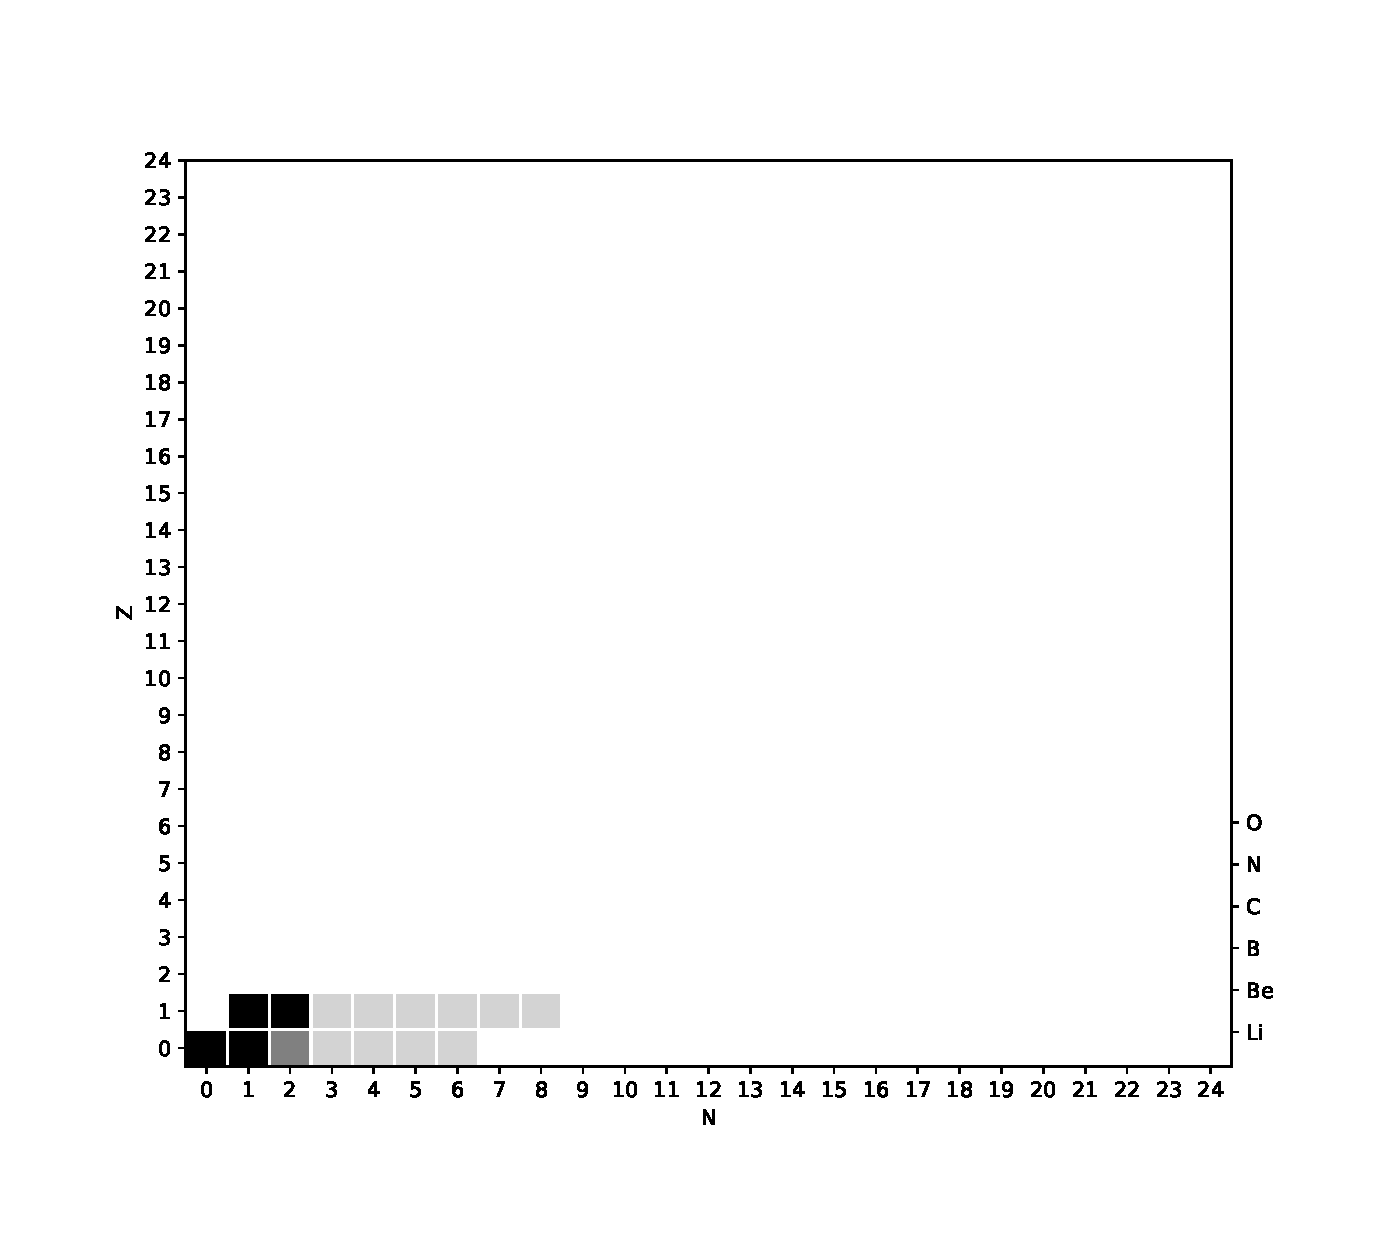
\includegraphics[scale=0.4]{images/atom_stability}
   \caption{Фрагмент диаграммы стабильности атомов химических элементов в зависимости от числа протонов и нейтронов в ядре. Темные клетки - стабильные атомы, светлые - относительно стабильные атомы, живущие от часов до миллиардов лет, пустые - нестабильные атомы, живущие не более малых долей секунд.}
   \label{fig:atom_stability}
\end{figure}




Электроны и протоны являются носителями электрического заряда, нейтроны электрически нейтральны. 
Электроны отрицательно заряжены, протоны - положительно, причем заряд электрона равен заряду протона, а числа электронов и протонов в атоме равны, так что атом оказывается электронейтральным в целом.
Бывает, что атом теряет или приобретает электроны, приобретая таким образом заряд и новое название - ион.
Здесь нас будут интересовать только атомы, не имеющие заряда.

При массе атома от $1.7\cdot 10^{-27}$ кг (атом Водорода-1) до $209.6\cdot 10^{-27}$ кг (атом свинца-208) масса одного электрона составляет всего $9.1\cdot 10^{-31}$ кг.
То есть в ядре сконцентрировано более $99.9\%$ всей массы атома.
Интересно, что кварки, из которых состоят протон, дают менее $2\%$ его массы, основная же часть массы протона приходится на виртуальные частицы.
Нам далее не потребуются столь глубокие субатомные понятия, как кварки и виртуальные частицы. 
Многие из них были открыты и изучены уже после Манхэттенского проекта и никак на него не повлияли. 


\section*{Цепные реакции}

Химические превращения одних веществ в другие происходят только путем перегруппировки атомов между их молекулами.
В процессе химической реакции молекулы исходных веществ отдают или принимают атомы, в результате образуя молекулы новых веществ. 
Сами атомы при этом остаются неизменными.
В этом смысле атом действительно является \textit{наименьшим} носителем химических свойств данного вещества, как и думали древние.

Таким образом, одних простых химических реакций недостаточно, чтобы решить главную задачу алхимии - заставить атомы одного вещества стать атомами другого.
Для того чтобы атомы одного вещества превратились в атомы другого, необходимо более грубое физическое вмешательство - ядерные реакции, в процессе которых ядра атомов взаимодействуют друг с другом или с элементарными частицами.
В результате ядерных реакций тяжелые атомы могут распадаться в более легкие (реакции деления), либо соединяться в еще более тяжелые (реакции синтеза).
Оба этих типа реакций происходят с выделением огромного количества тепла и радиации, что и послужило главной причиной для использования их в военных целях.

------------------------

сколько энергии выделяется при арспаде одного этома...


\section*{Уравнение Шреддингера}

Эта секция ... не важна для общего опнимания ....

УШ - чисто математический объект, причем весьма непростой.

Итак, откуда же можно получить хотя бы вероятность нахождения электрона в заданной области пространства?
Оказывается, она может быть найдена точно как решение уравнения Шреддингера

\begin{equation}\label{eq:schroedinger_1}
\nabla\psi + \frac{2m}{\hbar^2}(E - U(x))\psi = 0.
\end{equation}

Решения этого уравнения $\psi(x)$ комплекснозначны, но физический смысл имеют только их модули. 
Не вдаваясь в технические детали, можно сказать, что уравнение (\ref{eq:schroedinger_1}) дает искомую плотность вероятности обнаружения электрона в точке $x$ как квадрат модуля функции-решения $|\psi(x)|^2$.
Подробнее об уравнении Шреддингера можно почитать в приложении ....

\begin{figure}[t!]
   \centering
   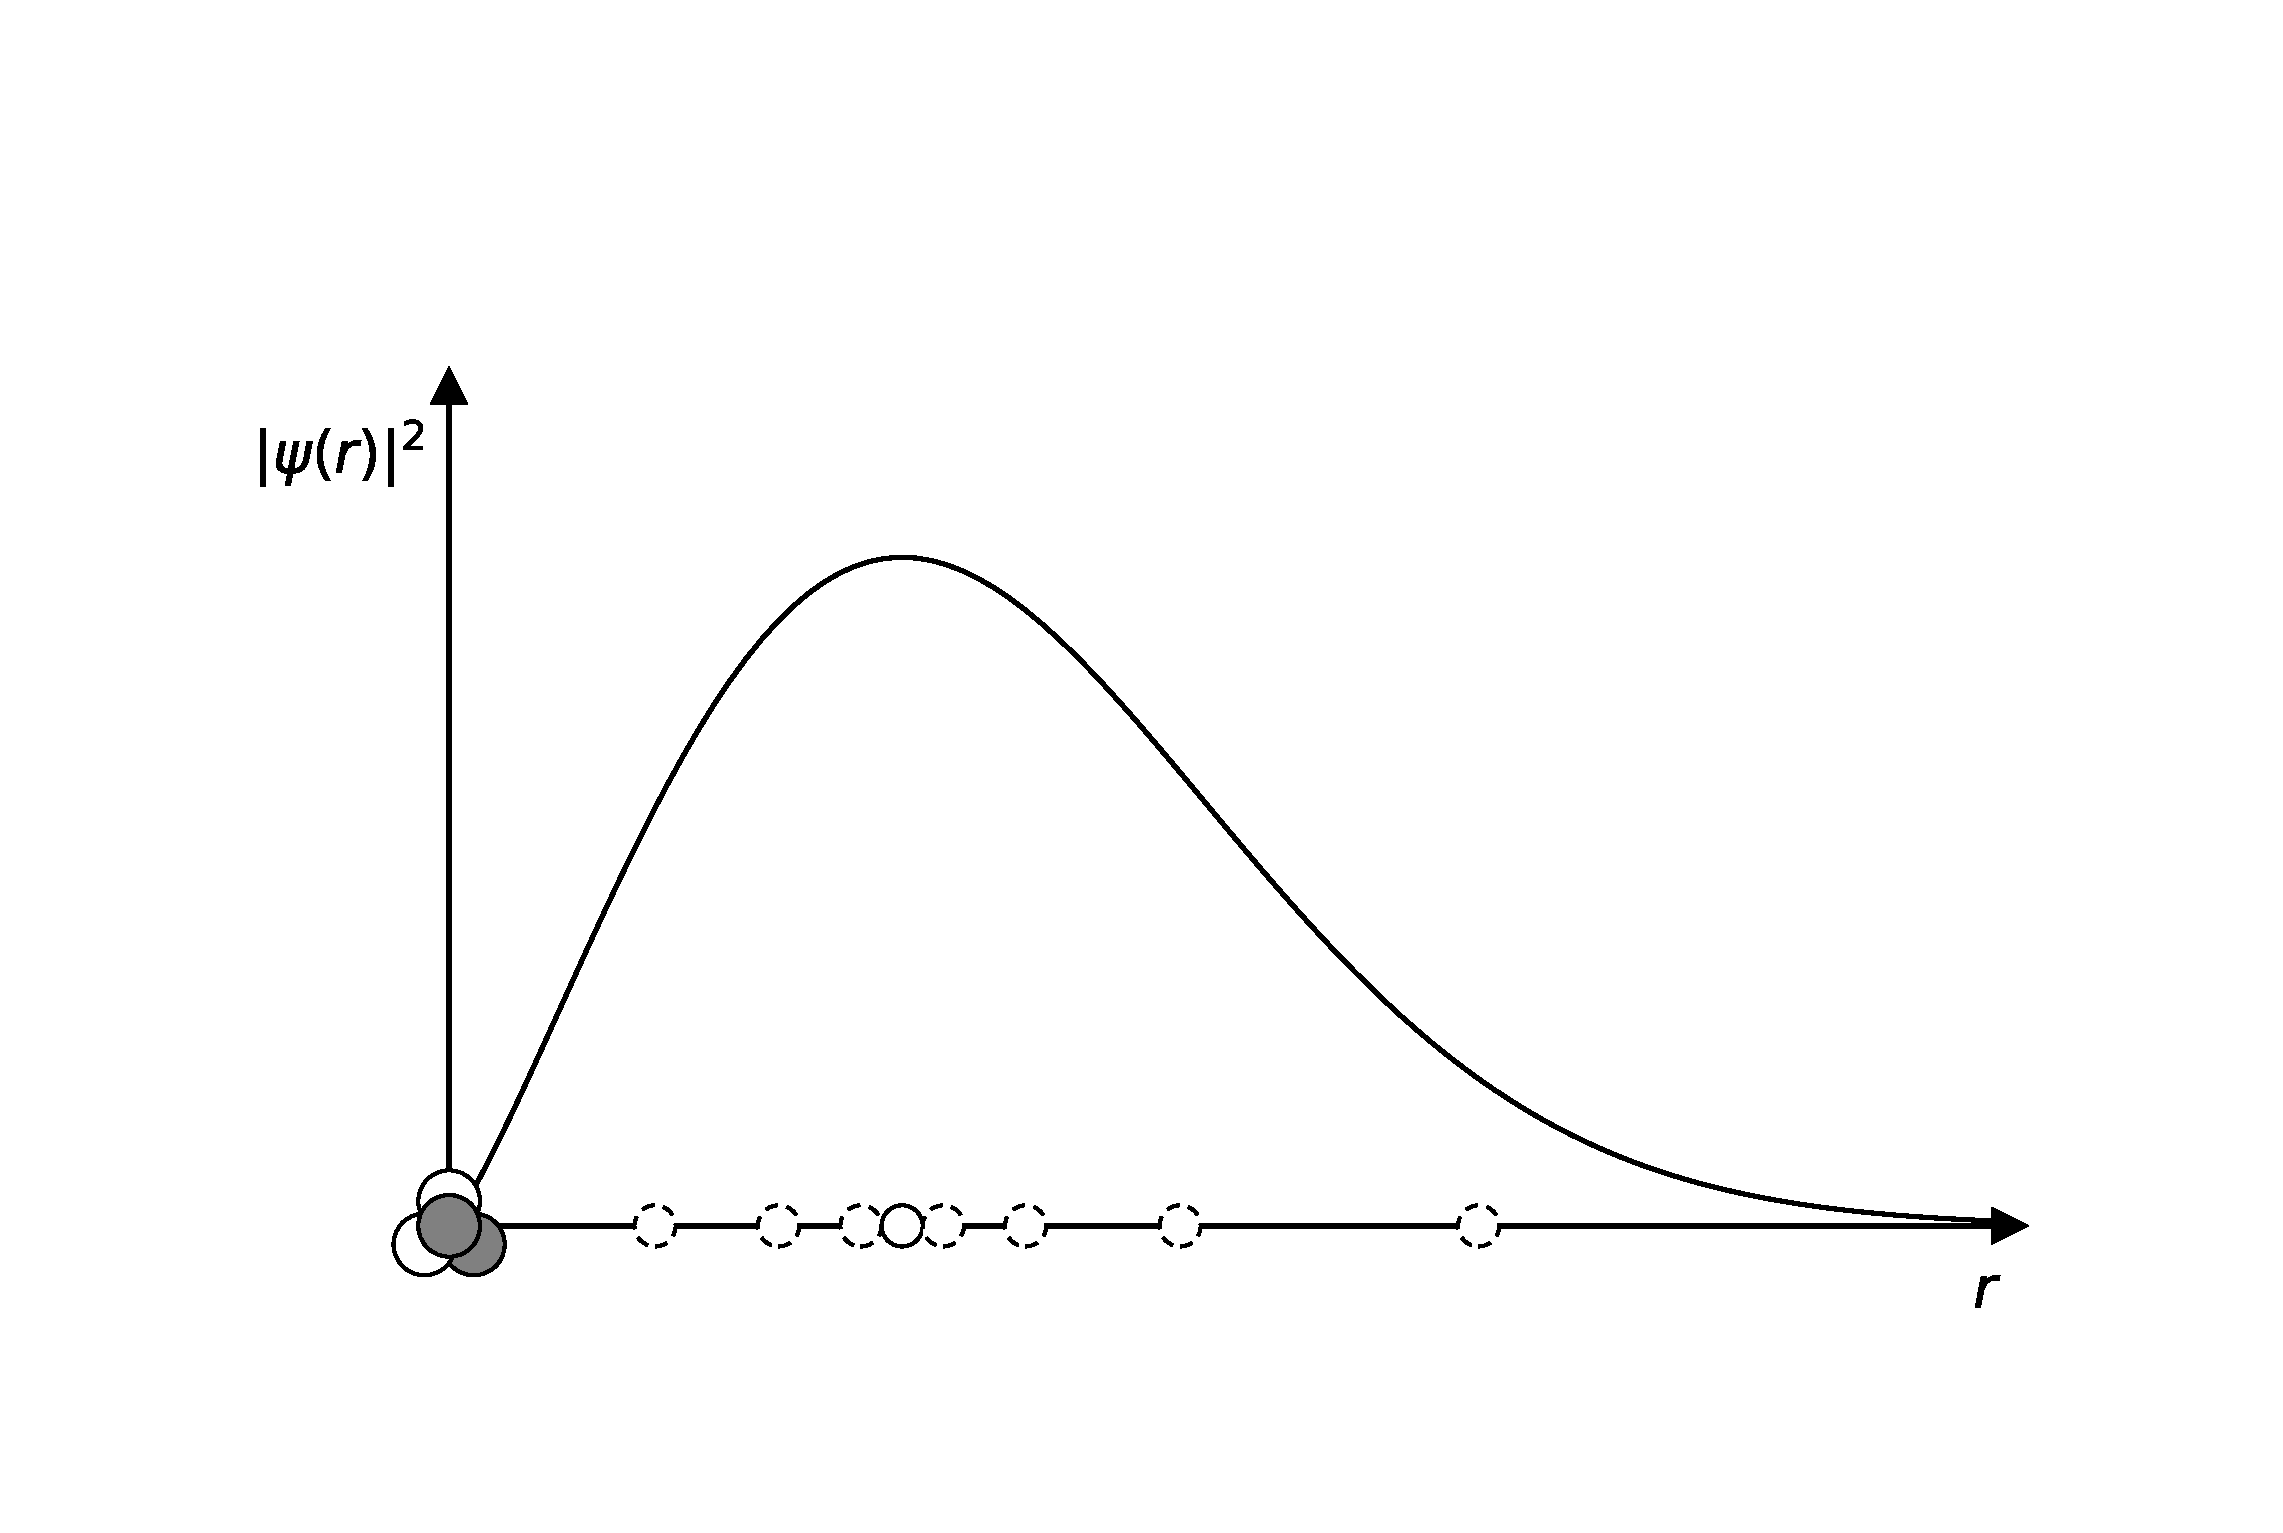
\includegraphics[scale=0.4]{images/radial_prob}
   \caption{Сферически симметричная плотность вероятности местонахождения электрона атома гелия как функция расстояния $r$ до ядра. Электрон может находиться не только в наиболее вероятном месте - точке максимума плотности, но и вообще в любом месте, хотя и с меньшей вероятностью.}
   \label{fig:radial_prob}
\end{figure}


------------------------ IDEAS ------------------------ 

По словам Эйнштейна, ``воображение важнее знания, так как знание ограничено''.
В XX веке теории об атоме предстояло пережить... что даже воображение не всегда справлялось...


Атом вполне может приобретать или терять электроны, получая таким образом заряд и становясь \textit{ионом}.
Порцессы ионизации в ядерных реакциях нас не 



атомы - интуиция еще со времен древних греков, но дальше - перерыв почти на x000 лет связанный с тем, что увидеть объект своих измышлений уже не возможно.
прорыв - с появлением соответсвующих средств измерений, но тут ученых ждал очень большой сбрприз
до этого схема научных открытий в большинстве своем состояла в следующем - смотрели, измеряли, придумывали теорию основнную на уже известных аналогиях, потом совершенствовали приборы, и снова смотрели и придумывали анлогию и т.п.
в атомной физике известных аналогий не нашлось. Наблюдения зачастую в корне противоречили известным фактам о макромире. Любая попытка смотреть на макро-аналогии заканчивалась появлением множества противоречий теории с экспериментом и в конце концов полным провалом 


физика - ранее умение делать открытия зависело от того, насколько наблюдателен был ученый, насколько хорошо он умел проводить параллели между уже известными ялениями и только изучаемыми.
Движения огромных небесных тел описывалось исходя из аналогичных движений, которые можно было повторять в удобном масштабе в своей алборатории и т.п. [еще примеры]
Новая физика потребовала от ученых вообразить нечто не имевшее аналогов с ранее изученным в принципе. 
Это восхищало даже далеких от физики современников.
В математике такие штуки привыкли проворачивать довольно давно. 
Стефан Банах, один из создателей современной математики в ее [современном] виде, говорил "Хорошие математики видят аналогии, лучшие могут видеть аналигии между аналогиями". Сам он, безусловно, был одним из лучших.

 
слова "теория относительности", "квантовая механика" носились в воздухе. Их можно было слышать  понимающих и истолковыва

----------------------------



https://ru.wikipedia.org/wiki/%D0%AD%D0%BB%D0%B5%D0%BA%D1%82%D1%80%D0%BE%D0%BD%D0%BD%D0%B0%D1%8F_%D0%BF%D0%BB%D0%BE%D1%82%D0%BD%D0%BE%D1%81%D1%82%D1%8C
{
В качестве модели состояния электрона в атоме, в квантовой механике принято представление об электронном облаке, плотность соответствующих участков которого пропорциональна вероятности нахождения там электрона.

Электронное облако часто изображают в виде граничной поверхности. При этом обозначение электронной области при помощи точек опускают. Пространство вокруг ядра, в котором наиболее вероятно пребывание электрона, называют атомной орбиталью (смысл которого вытекает из волнового уравнения Шрёдингера).

Применяются графические изображения распределения электронной плотности относительно ядра.

Кривая радиального распределения вероятности показывает, что электрон находится в тонком концентрическом шаровом слое радиуса r толщины dr вокруг ядра атома водорода[1].

Проекция максимума кривой соответствует боровскому радиусу alpha_0=0,53 A_with_circle.

Во многих случаях для решения уравнения Шрёдингера используют различные приближения. Вероятностную (статистическую) интерпретацию волновой функции разработал Макс Борн. В 1954 году М.Борн удостоен Нобелевской премии по физике с формулировкой «За фундаментальные исследования в области квантовой механики, особенно, за статистическую интерпретацию волновой функции.»
}

https://ru.wikipedia.org/wiki/%D0%A1%D1%82%D0%B0%D1%82%D0%B8%D1%81%D1%82%D0%B8%D1%87%D0%B5%D1%81%D0%BA%D0%B0%D1%8F_%D0%B8%D0%BD%D1%82%D0%B5%D1%80%D0%BF%D1%80%D0%B5%D1%82%D0%B0%D1%86%D0%B8%D1%8F_%D0%B2%D0%BE%D0%BB%D0%BD%D0%BE%D0%B2%D0%BE%D0%B9_%D1%84%D1%83%D0%BD%D0%BA%D1%86%D0%B8%D0%B8
{
М. Борн вспоминал:
Он (Шрёдингер) рассматривал электрон не как частицу, но как некоторое распределение плотности, которое давалось квадратом его волновой функции |ψ|².

Он считал, что следует полностью отказаться от идеи частиц и квантовых скачков, и никогда не сомневался в правильности этого убеждения. Я, напротив, имел возможность каждодневно убеждаться в плодотворности концепции частиц, наблюдая за блестящими опытами Франка по атомным и молекулярным столкновениям, и был убеждён, что частицы не могут быть упразднены. Следовало найти путь к объединению частиц и волн. Я видел связующее звено в идее вероятности…
}



\chapter{Проект ``Манхэттен''}\label{ch:manhattan_project}

\epigraph{\emph{Каждое орудие несет в себе дух, \break благодаря которому оно создано.}}
{Вернер Гейзенберг}

TODO

------------------------ IDEAS ------------------------ 

персоналии физики
персоналии математики, Львовская школа и т.п.

\chapter{Бомба}\label{ch:the_bomb}

\epigraph{\emph{Если у тебя есть оружие, \break скоро ты найдешь предлог им воспользоваться.}}{Стив Айлетт}

TODO

------------------------ IDEAS ------------------------ 

http://nuclphys.sinp.msu.ru/enc/e198.htm

https://ru.wikipedia.org/wiki/%D0%9E%D0%B1%D0%BE%D0%B3%D0%B0%D1%89%D0%B5%D0%BD%D0%B8%D0%B5_%D1%83%D1%80%D0%B0%D0%BD%D0%B0
Причины обогащения - хорошие слова

\chapter{Зачем нужна математика?}\label{ch:why_math}

\epigraph{\emph{Каждая включенная в книгу формула \break уменьшает число ее читателей вдвое.}}{Стивен Хокинг, Роджер Пенроуз}

TODO

------------------------ IDEAS ------------------------ 

На этом подготовительную часть книги можно считать законченной.
Мы знаем, какие физические процессы стоят за созданием атомного оружия ([стоит ли упирать на оружие]) и в целом понимаем суть связанных с этим задач.
Мы представляем, какая работа была у физиков....
Что же делали математики? ....


Прежде чем пытаться разобраться в конкретных уравнениях и моделях, полезно значть в целом, а что же вообще способна дать математика?


Дмитрий Иванович Менделеев утверждал, что наука начинается там, где начинают считать

Математика - это организованные рассуждения

\chapter{Дифференциальные уравнения}\label{ch:differenrial_equations}

\epigraph{\emph{.}}{}

Уравнения являются одним из центральных объектов исследования в математике.
Составлять и решать простейшие уравнения нас учат еще со средней школе.
Там же мы знакомимся с многочисленными примерами того, где это может пригодиться.
Навыки записи и решения уравнений используется далее, в основном, в курсе школьной физики, где уравнения служат основным инструментом записи законов природы.

Не является исключением и более сложная ядерная физика, где все основные законы деления ядер записываются в виде уравнений, впрочем, куда более сложных, чем те, которые решаются в школе.
Эти уравнения носят название \textit{дифференциальных} и выражают зависимость скорости изменения некоторой величины (например, количества быстрых нейтронов в бомбе в данный момент времени) он нее самой. 
Решениями таких уравнений будут в свою очередь уже не отдельные числа, а функции, то есть зависимости одних величин от других.

Дифференциальные уравнения служат неиссякаемым источником истереснейших задач в самой математике и крайне полезны в прикладных науках. 
Они являются прочным мостом, связывающим чистую математику с прикладными науками и, в частности, теоретической физикой. 
Не будет преувеличение сказать, что вся классическая и современная физика говорят на языке дифференциальных уравнений.

В данной главе мы постараемся от простейших школьных уравнений подойти к дифференциальным, продемонстрировав их силу и суть. 


\section*{Числовые уравнения} 

Обычные уравнения, знакомые нам со школьной скамьи, обычно возникают напрямую из текстовых задач.
Обозначая неизвестные величины буквами и следуя условию задачи, мы переписываю ее в виде одного или нескольких уравнений, решая которые мы и находим все неизвестные.
Рассмотрим несколько примеров.

Пусть в процессе столкновения и последующего распада тяжелого ядра один нейтрон порождает $3$ новых нейтрона, которые далее без потерь делают то же самое.
Кроме того известно, что в системе включен постоянный источник нейтронов, дающий четыре нейтрона в единицу времени.
Требуется узнать, сколько нейтронов было в предыдущий момент, если в данный момент времени в системе имеется $100$ быстрых нейтронов.
Вводя неизвестную $x$ - число нейтронов в предыдущий момент времени, и идя по условию задачи, получаем соотношение
$$
3x + 4 = 100,
$$
представляющее собой простейшее линейное уравнение относительно неивестной $x$ с решением $x = 32$.

В процессе решения задачи вполне могут получиться и более сложные уравнения, нежели линейные.
Заметим, что в условии предыдущей задачи мы предположили, что ядерного топлива для деления у нас имеется неограниченное количество.
Такое предположение справедливо только на самых ранних этапах ядерной реакции и не имеет места, когда нейтроном становится слишком много, и топливо выгорает.
Иными словами, с течением времени не три, а все меньшее количество нейтронов будет встречаться с тяжелыми ядрами, вызывая последующий их распад.
Предположим, что топлива у нас осталось немного, и коэффициент размножения нейтронов не постоянен, а уменьшается в зависимости от числа нейтронов $x$ как $3 - 0.1x$. 
Найдем, сколько нейтронов было в системе в предыдущий момент, если в данный момент времени в системе имеется $204$ быстрых нейтрона.
Составляя уравнение согласно условию задачи, получим
$$
(3 - 0.01x)x + 4 = 104.
$$
Вспоминая школьные формулы решения квадратных уравнений, получаем $x = 100$ или $x = 200$.
Оба решения имеют физический смысл.
Без дополнительных условий мы не можм сказать, сколько нейтроном было из начально - $100$ или $200$.

Сделаем несколько важных замечаний. 
Во втором примере мы усложнили модель, включив эффект иссякания ресурсов и сделав тем самым ее более приближенной к реальности.
И сразу же усложнилось уравнение, описывающее задачу.
Оно стало нелинейным и дало два возможных решения вместо одного.
Позже мы увидим, что максимально приближенные к реальности модели вообще не могут быть решены в явном виде.
Их приходится исследовать качественно, либо численно.

Пойдем далее.
Предположим, нас интересует поведение количества нейтронов не в один фиксированный момент времени, а во все сразу.
Таким образом, интересует поведение этой величины с течением времени: будет ли число нейтронов в системе возрастать, либо убывать.
Проще говоря,... основной вопрос, который волновал ученых Манхэттенского проекта - произойдет ли взрыв?

Предположим, что мы отуда-то знаем, что коэффициент размножения участвующих в реакции нейтронов постояннен (на время пренебрежем эффектом выгорания топлива) и равен некоторому числу $k$.
Если в начальный момент времени $t=0$ в системе было $x_0$ нейтронов, то в последующий будет $kx_0$, затем $k^2x_0$ и так далее.
В момент времени $t$ количество нейтронов в системе будет равно
\begin{equation}\label{eq:simple_neutron}
x_t = k^tx_0.
\end{equation} 
Что нам дает соотношение (\ref{eq:simple_neutron})?
Во-первых, оно позволяет при известном начальном количестве нейтронов и коэффициенте размножения вычислить число нейтронов в любой момент времени.
Во-вторых, оно позволяет решать и обратные задачи: находить, каким было изначальное число нейтронов, либо коэффициент размножения, если известно их количество в другие моменты.
И наконец, в-третьих, соотношение (\ref{eq:simple_neutron}) позволяет \textit{качественно} оценить поведение в системе в целом: при $k<1$ количество нейтронов в системе будет становиться все меньше и меньше, а при $k>1$ будет неограниченно возрастать - произойдет взрыв.

Минус модели (\ref{eq:simple_neutron}) - ее неточность.
Хоть она и дает число нейтронов в любой момент времени, но это число будет не точным из-за слишком больших упрощений, сделанных при ее выводе.
Постараемся учесть эффект выгорания топлива, как это было сделано в примере 2 выше.




В школьной программе, впрочем, довольно близко подходят к этому.
Уравнения с параметром

Дифференциальные уравнения - зависимость производной величины от нее самой

История
 

\chapter{Самообучаемые алгоритмы}\label{ch:self_learning_algorithms}

\epigraph{\emph{.}}{}

Манхэттенский проект оказал значительное влияние на физику, математику и науку в целом.
Его населедие огромно.
Ряд подходов и целых областей современной науки родились в стенах Лос-Аламосской национальной лаборатории и затем бурно развивались, давая все новые плоды уже вне области создания ядерного оружия.

Одним из самых главных прикладных достижений проекта, сыгравшем решающую роль в его успехе, было упор на математическое и компьютерное моделирование всех необходимых физических процессов.
Это было немыслимо без мощных вычислительных машин, что в итоге определило последовавшую глобальную компьютеризацию всех областей человеческого знания.
Сначала все расчеты для Проекта велись силами целой команды \textit{human computers} - девушек-вычислителей, вручную делавших все арифметические опреации.
Руководил командой Ричард Фейнман, ставивший перед вычислителями задачи по решению сложных дифференциальных уравнений, описывающих процесс взрыва бомбы.
Очень скоро стало понятно, что уравнения сложны настолько, что использование человеческого труда становится попросту неоправданно.   
Это была поворотная точка, когда для сложных и ответственных расчетов стали использоваться компьютеры, тогда еще совсем примитивные.

К слову, некоторые из вычислителей, выполнявших до этого всю работу вручную, затем переквалифицировались для работы с новыми вычислительными машинами.
Первые шестеро программистов ЭНИАКа (первого серьезного компьютера) были именно теми самыми девушками-вычислителями [???], выполнявшими ранее всю работы 
Шесть

Развитие компьютеров стремительно развивалось сразу по нескольким направлениям.
Во-первых, развивалась сама архитектура устройств, позволяя сократить их размеры с компьютеров размером в небольшой стадион до размеров, вполне сравнимых с сегодняшними.

Во-вторых, возрастали вычислительные мощности компьютеров.
Если сначала они были сравнимы с мощностями нескольких людей-вычислителей [???], то уже через несколько лет [???]

Наконец, упрощалось само взаимодействие человека с вычислительной машиной.
Изначально выполнение даже простейших задач на компьютере было доступно лишь специалистам высочайшего класса.
Это было сделано отчасти осознанно, так как предполагалось, что подобные разработки могут пригодиться только военным, а следовательно уровень доступа к ним должен быть соответствующий.
Как говорили в свое время создательнице первого в истории компилятора*  Грейс Хоппер, “Но Грейс, ведь тогда любой сможет писать программы!”.

Сегодня компьютерные программы действительно может писать любой человек. 
Более того, подобный навык все чаще фигурирует как прямое требование при приеме на работу на самые разные должности.
Сегодня умение писать программы становится неотъемлемой частью человеческой культуры.
А истоки этого идут именно от МП.

Можно было бы много и долго перечислять конкретные достижения компьютеризации, начало которым было положено в МП.
Остановимся здесь на самой “горячей” в последние годы теме - машинном обучении и искусственном интеллекте.
Эти области на первый взгляд не имеют прямого отношения к МП.
Мы выбрали здесь именно эту область скорее для демонстрации того, какую форму могут принять правильно и вовремя поданные идеи.
Такой идеей было повсеместное использование вычислительных машин для моделирования различных процессов реального мира.

## Самообучающиеся алгоритмы

[пример: дерево и кастомные фильтры изображений]

## Проблемы обучения

[недообучение]
[переобучение - пример со студентами, реальный пример]
[обобщающая способность]

## Примеры приложений

## Общая постановка задачи

[постановка]









Новый тип алгоритмов

------------------------ IDEAS ------------------------ 


\begin{thebibliography}{9}

\bibitem{bib_mathphylhist} 
Радул Д.Н. 
\textit{История и философия науки: философия математики}. 2-е изд., испр. и доп. Учебное пособие для вузов. 2019.

\bibitem{bib_archimed} 
Архимед.
\textit{Сочинения}. М., 1962.

\bibitem{bib_feynmanphyslaws} 
Фейнман Р.
\textit{Характер физических законов}. М.: Издательство АСТ, 2018.

\bibitem{bib_lomonosov} 
Ломоносов М.В.
\textit{Полное собрание сочинений}. Изд. АН СССР, М.-Л., 1951

\bibitem{bib_lomonosov} 
Арнольд В.И.
\textit{Истории давние и недавние}. М., ФАЗИС, 2002.

\bibitem{bib_chemhist} 
Левченков С.И.
\textit{Краткий очерк истории химии}. Ростов н/Д: Изд-во Рост. ун-та, 2006.

\bibitem{bib_antique_philosophy} 
Шишкоедов П.
\textit{Философия античности}. Издательские решения, 2015.

\bibitem{bib_democrit} 
Лурье С.Я.
\textit{Демокрит}. Л.: Наука, 1970.

\bibitem{bib_ancient_atomism} 
Лурье С.Я.
\textit{Теория бесконечно малых у древних атомистов}.  М.-Л.: АН СССР, 1935.

\bibitem{bib_chemistry} 
Третьяков Ю.Д., Олейников Н.Н., Кеслер Я.А., Казимирчик И.В.
\textit{Химия: справочные материалы}. М.: Просвещение, 1989.

\bibitem{bib_antique_philosophy} 
Шамшин Д.Л.
\textit{Химия: Учеб. пособие}. М.: Высшая школа, 1980.

\bibitem{bib_niels_bohr_1} 
Niels Bohr
\textit{The Philosophical Writings of Niels Bohr}. Ox Bow Press, 1987

\bibitem{chem_basics} 
Мануйлов А.В., Родионов В.И.
\textit{Основы химии для детей и взрослых}. М.: Центрполиграф, 2018 г.

\end{thebibliography}


\end{document}
